% Setup
\documentclass[a4 paper, 12pt]{article}

% Title
\title{COSC3000 - COMPUTER GRAPHICS REPORT \\ --- \\OLYMPIC STADIUM}
\author{Tean-louise Cunningham (42637460)}
\date{\today}

% Margins
\usepackage{geometry}
\geometry{margin=2cm}

% Images
\usepackage{graphicx}
\usepackage{float}
\usepackage[export]{adjustbox}
\setlength{\intextsep}{5pt plus 2pt minus 2pt}
\usepackage[font=small,skip=3pt]{caption}


% Paragraph
\setlength{\parindent}{0em}
\setlength{\parskip}{1em}

% Text Formatting
\usepackage[utf8]{inputenc}
\usepackage[english]{babel}

% List spacing
\usepackage{enumitem}
\setlist{noitemsep, topsep=0pt}
\setlist[enumerate]{parsep=5pt} 

% Text Color
\usepackage{xcolor}

% Hyperlinks
\usepackage{hyperref}
\hypersetup{
    colorlinks=true,
    linkcolor=black,
    filecolor=black,      
    urlcolor=blue,
}

% Appendix
\usepackage{appendix}

% Include pdf
\usepackage{standalone}
\usepackage{pdfpages}

% Borders
\usepackage{mdframed}

% Appendix
\usepackage{appendix}

% Code
\usepackage{listings}
\definecolor{backcolour}{rgb}{0.95,0.95,0.92}
\lstset{basicstyle=\footnotesize, language=python, backgroundcolor=\color{backcolour}}

% Remove number from sections
\setcounter{secnumdepth}{0}

\usepackage{multicol}
\usepackage{amssymb}
\usepackage{standalone}
\usepackage{pdfpages}

%%%%%%%%%%%%%%%%%%%%%%%%%%%%%%%%%%%%%%%%%%
% DOCUMENT
\begin{document}

% Title
\maketitle
    \begin{figure} [H]
        \centering
        \includegraphics[width=0.95\textwidth]
            {./images/title.png}                  
    \end{figure}  


% Table of contents
\pagebreak
\tableofcontents
\pagebreak
\listoffigures


% INTRODUCTION
\pagebreak
\section{Introduction}
In continuance of the exploration of the Olympics from the visualisation project, a graphic simulation of running on an athletic track will be simulated. The main stadium of an Olympics is the most integral location as it hosts the opening and closing ceremonies, the lighting of the touch and the most popular events [19]. The architecture and design choices of these stadiums ensure athletes can compete in optimal circumstances and thousands of spectators can experience these feats [18]. This project will highlight the ingenuity of these stadiums by offering the opportunity to view its design in detail as a competitor on its athletic track. The end goal is to have a model of an athlete posed as running able to move along an athletic track surrounded by stadium seating and accompanied by props. 

In order to achieve this goal all of the tier 1 deliverables for the provided mega\_racer project were first implemented, as well as the tier 2 tasks of improving terrain texture, adding fog and props. Once these steps were successfully implemented, the base mesh of a human model was rigged and posed, and clothing models textured and set on the model. The models of the Olympic Rings and a safety cones were created as props, appropriate textures mapped and a new map to represent the shape of a stadium was created. To complete all of these tasks various Computer Graphics concepts and techniques were demonstrated, including coordinate systems, setting up a virtual camera, lighting, shading, texturing and modelling in Blender. This report aims to document and communicate the process and understanding of these concepts. The provided self-contained pre-package distribution for Windows is used to run all code in this project.

The presentation of this project can be viewed \href{https://youtu.be/X3s_5GrY3Jw}{here}, in addition to the code \href{https://drive.google.com/drive/folders/13qEjRWL_FDgG3QQQaAF3BSkbr69Wab3i?usp=sharing}{here}.

% MEGA RACER
\section{Mega Racer}
Mega Racer is a basic game simulating a race car driving through a wilderness area. The basic game logic, movement and sun light has been provided in the code. Additionally, examples files for the object models, textures and map have been provided and were used for this implementation. There are two tiers of task; basic and advanced. All of the tier 1 tasks were completed successfully as well as the first three tasks from tier 2; improved terrain textures, and the addition of fog and props. These tasks provided a strong foundation for the proposed implementation of an Olympic Stadium in the next section. 

%% TIER 1
\subsection{Tier 1}
These are the basic deliverables that highlight a basic understanding of computer graphic techniques. There are five tasks all of which were completed in the provided code and accompanied here with explanations, screenshots and the relevant code. The provided code produces the world space coordinate system however there are no objects yet in the world.

%& 1.1
\subsubsection{1.1 - Scale the terrain grid}
The map of the world is a RGB image for simplicity. Fundamentally this image is simply a grid of pixels, each of which is an addressable colour sample [43]. The provided map and game logic relies on the value of the red pixel to indicate the height of the terrain, with 255 as the maximum height. The provided code normalises the R pixel value by dividing it by this maximum value to be a value between 0 and 1, and assigned as 'red'. By multiplying this variable with the provided uniform scaling variable, heightScale, all axis will be scaled to the appropriate units of the world space, in this case 75 metres, for a realistic appearance [44]. This operation is assigned to the zPos of the terrain when it loads in terrain.py to set the height, as well as uncommenting the last line from racer.py so the racer can follow the height.   
    \begin{lstlisting}
# terrain.py
def load(...):
    ...
    zPos = red * self.heightScale
    ...
    \end{lstlisting}

    \begin{figure} [H]
        \centering
        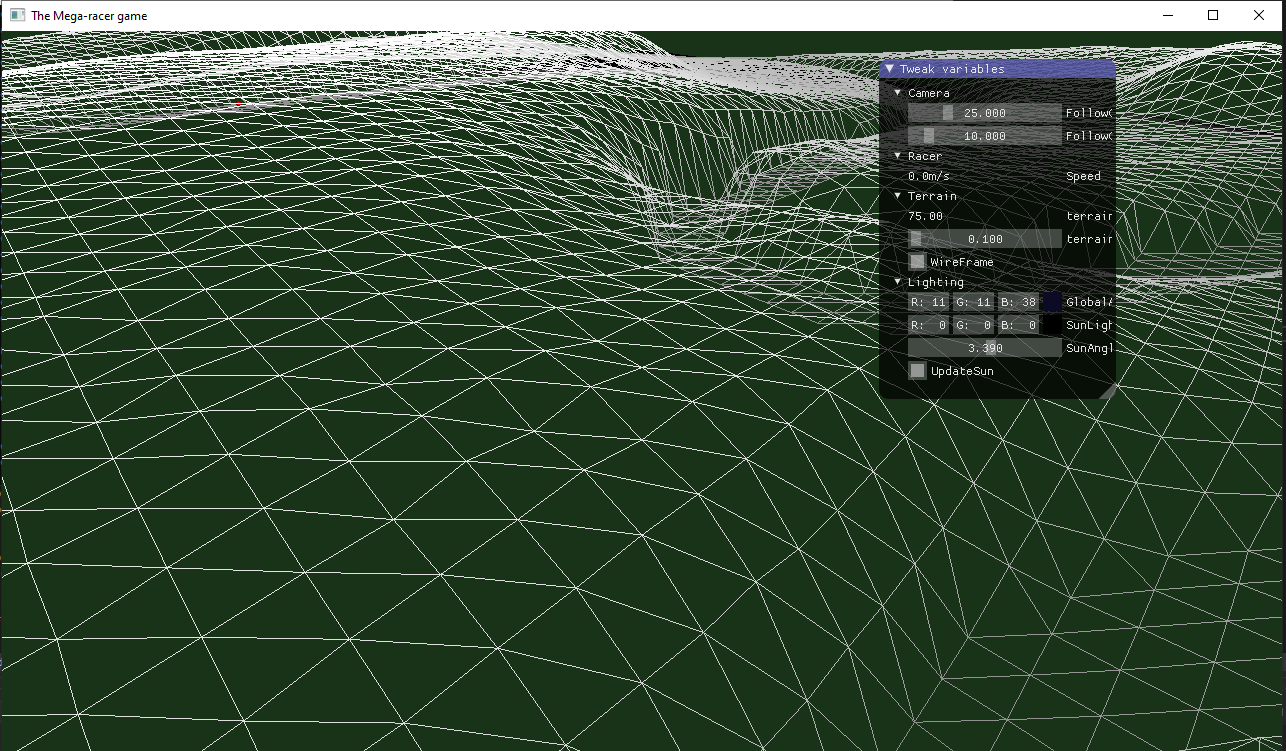
\includegraphics[width=0.8\textwidth, frame]
            {./images/mega_racer/1.1.PNG}
        \caption{1.1 - Scale the terrain grid}
    \end{figure}  
   

%% 1.2
\subsubsection{1.2 - Set up a camera to follow the racer}
In this task the coordinate system of the view space will be determined, as the view space is simply the space as seen by the camera. This coordinate system is the result of transforming the world space so that the object is in front of a users view, through a combination of translations and rotations [44]. In the code, there is a variable clearly labelled worldToViewTransform which is assigned the output of lu.make\_lookAt(). This function then calls lu.make\_lookFrom() with a modified target parameter for smooth movement. A very similar process is followed in the example from lab 2 [50]. 
    \begin{lstlisting}
# Lab 2 (1) - Q5, Lab 2 (2) 
worldToViewTransform = magic.make_lookAt(eyePos, [0,0,0], [0,1,0])
worldToViewTransform = magic.make_lookFrom(g_cameraPosition, cameraDirection, [0,1,0])

# mega_racer.py 
def renderFrame(...):
    ...
    view.worldToViewTransform 
        = lu.make_lookAt(g_viewPosition, g_viewTarget, g_viewUp)
-->
# lab_utils.py
def make_lookAt(eye,target,up):
    return make_lookFrom(eye, np.array(target[:3]) - np.array(eye[:3]), up)
--> 
def make_lookFrom(eye,direction,up):
    .....
    \end{lstlisting}

There are four key variables when creating a virtual camera; Up, Camera Position, View Direction and View Target. From the code, the meaning of each of the variables can be understood so they can be appropriately assigned so the world to view transformation is accurate. All of these variables are vectors with xyz coordinates and currently these variables only have default values.
    \begin{itemize}
        \item Up: In this case \textit{g\_viewUp} represents the rough up direction and, as commonly used, corresponds to the world up direction. This constrains the orientation of the view to avoid arbitrary roll, though it isn't perpendicular to the view direction (Lecture 3). This value does not need to be updated at any point after being globally declared.
        \item Camera Direction: The view direction of the camera is often in terms of another position or the view target i.e. where the camera is supposed to look. There is no specific variable relating to this concept, however it is calculated by subtracting the target (\textit{g\_viewTarget}) from the eye (\textit{g\_viewPosition}) variables in \textit{make\_lookFrom()}.
    \end{itemize}

In order for the camera view to be relative to the movement of the racer these values need to be modified in update().
    \begin{itemize}
        \item View Target: The racer is the target and so the corresponding variable, \textit{{}g\_viewTarget}, needs to be updated to the position of the racer with each movement of the racer as this where the camera needs to be pointing. Additionally, the z coordinate requires the addition of \textit{g\_followCamLookOffset} to offset the look target above the racer. 
        \item Camera Position: The position of the camera or the centre of projection is basically the the eye of the viewer, which in this case is the \textit{g\_viewPosition}.Since the desired view is that of above and behind the racer this variable needs to be updated to take into account corresponding position of the racer (view target), as well as the \textit{g\_followCamOffset} (behind and above) for all coordinates. This is achieved using vector addition to add the offset to the racer position.
    \end{itemize} 

\textbf{Attempt 1 - Direction Missing}: The result after running these changes performed the calculation of a view space coordinate system that now updated relative to the racer and was in a better position. However, the movement of the racer to the movement of the camera was the opposite and the rotation transformation was off. The camera position should have a relationship with both the view target and view direction, but the view direction has not been taken into consideration. 
    \begin{lstlisting}
# mega_racer.py
def update(...):
    ...
    g_viewTarget = g_racer.position.copy()
    g_viewTarget[2] += g_followCamLookOffset

    g_viewPosition = g_racer.position + (g_followCamOffset)
    g_viewPosition[2] += g_followCamOffset
    \end{lstlisting}

\textbf{Attempt 2 - Correct to specification}:
On closer inspection of the Racer class, \textit{heading} controls the direction of the racer. Since the camera needed to be behind the racer, the camera position (g\_viewPosition) had to be multiplied by the inverse of the racer direction using vector multiplication. This produced the correct result in relation to the position of the racer with the offsets applied at the appropriate direction to the racer's movement.

\begin{lstlisting}
# mega_racer.py
def update(...):
    ...
    g_viewTarget = g_racer.position.copy()
    g_viewTarget[2] += g_followCamLookOffset

    g_viewPosition = g_racer.position + (g_followCamOffset * -g_racer.heading)
    g_viewPosition[2] += g_followCamOffset
\end{lstlisting}

\begin{figure} [H]
    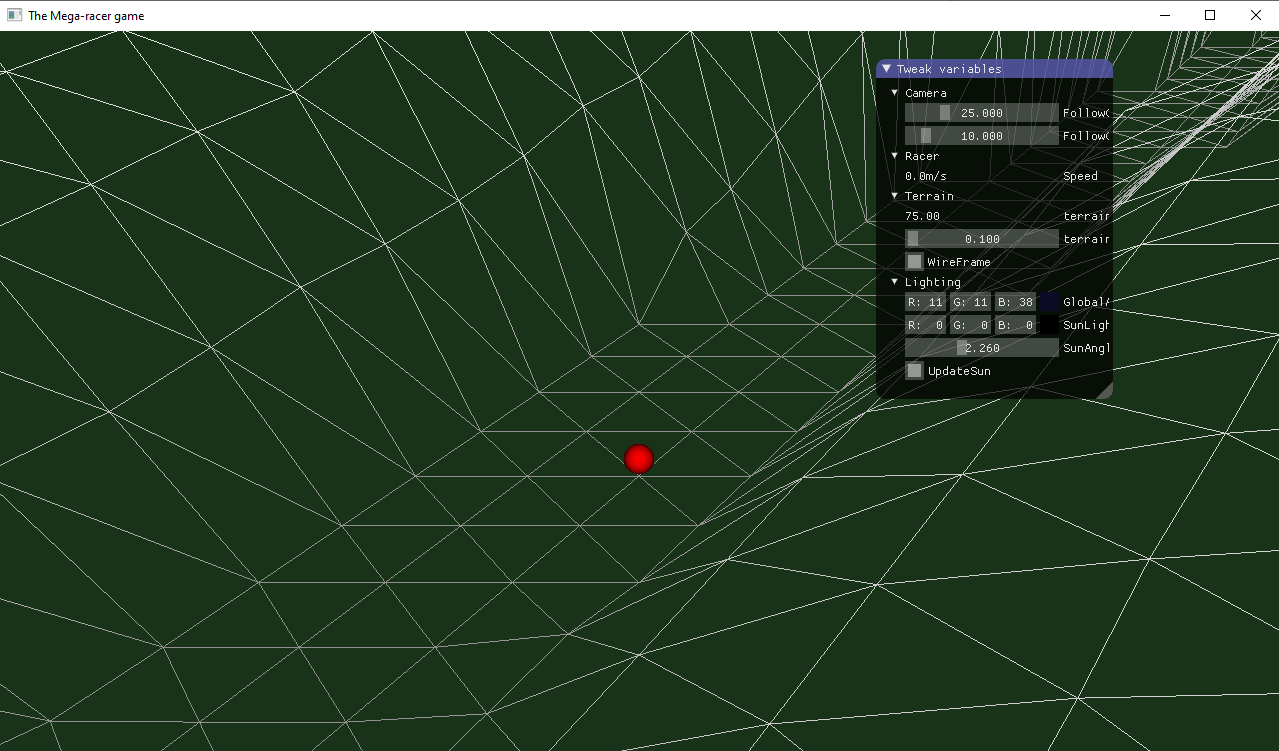
\includegraphics[width=0.49\textwidth, frame]
        {./images/mega_racer/1.2_1.PNG}
        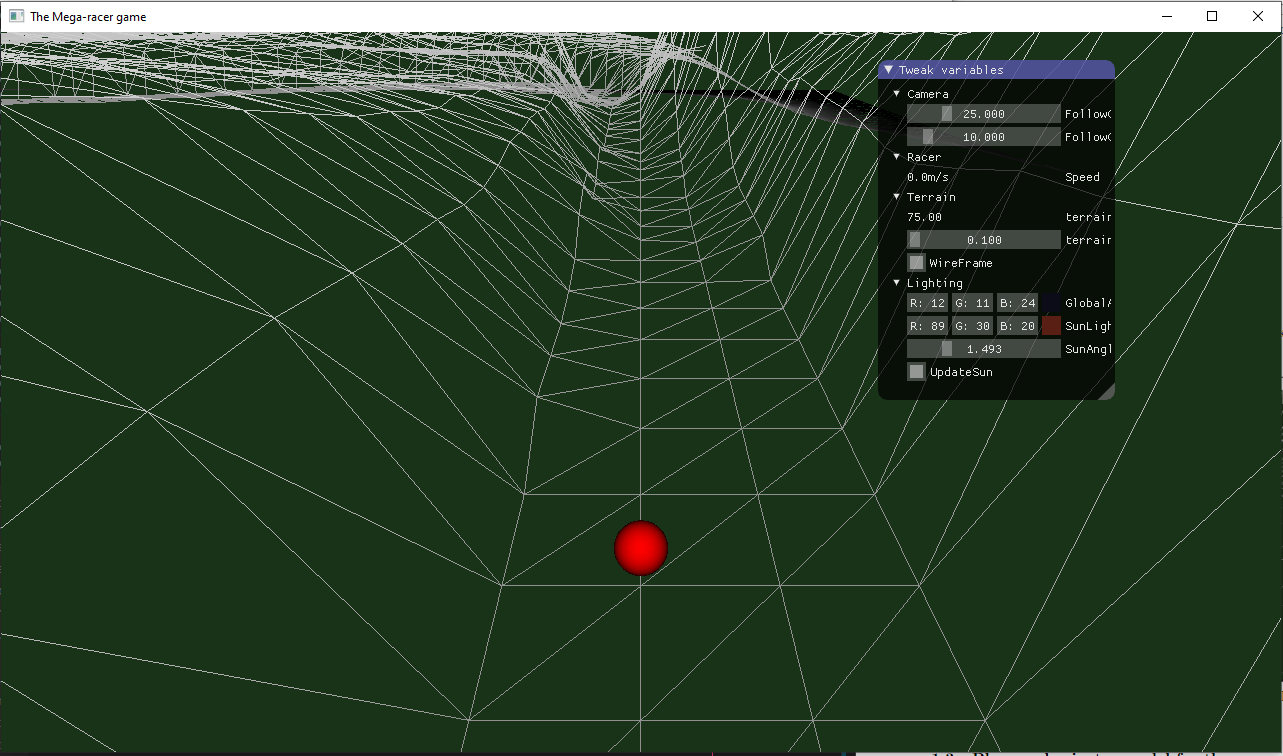
\includegraphics[width=0.49\textwidth, frame]
        {./images/mega_racer/1.2_2.PNG}
    \caption{1.2 - Camera follow racer - Attempts}
\end{figure}

Although the correct position was calculated, a more intimate view of the racer was desired. So instead the viewTarget was set to equal the racer's position, and the g\_followCamLookOffset was added to the z coordinate of the view position. This placed the camera at the same distance above and behind, but instead the racer is in the centre of the camera view. This achieves a view with the racer at centre of attention with good eye scan, unity and compositional balance [5,6] which provides the optimal camera view for the next section when modifying to the Olympic Stadium.
    \begin{lstlisting}
# mega_racer.py
def update(...):
    ...
    g_viewTarget = g_racer.position

    g_viewPosition = g_racer.position + (g_followCamOffset * -g_racer.heading)
    g_viewPosition[2] += g_followCamLookOffset
    ...
    \end{lstlisting}

    \begin{figure} [H]
        \centering
        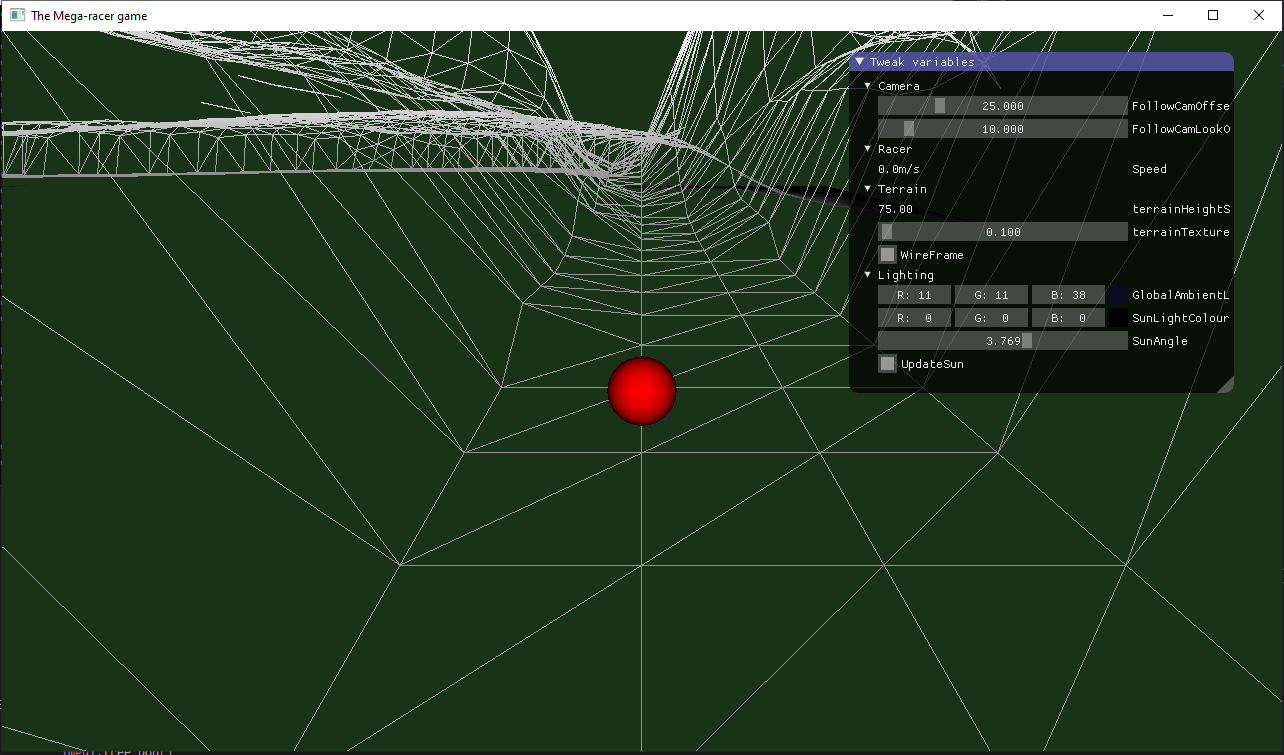
\includegraphics[width=0.8\textwidth, frame]
            {./images/mega_racer/1.2_b.PNG}
        \caption{1.2 - Camera follow racer - Final}
    \end{figure}  


%% 1.3
\subsubsection{1.3 - Place and orient a model for the racer}
This section follows the process of an object to world space transformation. The object space is the local coordinate system to the object (racer), where the object is centred at the origin. By transforming to the world space the object will be placed and able to move in this scene appropriately. To complete this transformation there are two functions that need to be updated in racer.py; render() and load(). 

\textbf{(1) Rendering the model}: In \textit{mega\_racer.renderFrame()} the racer is being rendered in the world by calling \textit{racer.render()}. This is where the model of the racer needs to be drawn. 
    \begin{lstlisting}    
# mega_racer.py
def renderFrame(...):
    ...
    g_racer.render(view, g_renderingSystem)  
-->
#racer.py - Racer
def render(self, view, renderingSystem):
    .....
    \end{lstlisting}  

To render the racer model, it must be drawn and replace the sphere. To draw the object, as per the project notes, \textit{renderingSystem.drawObjModel()} was used. The parameter, \textit{renderingSystem}, is of RenderingSystem class which provides access to \textit{drawObjModel()}. 
    \begin{lstlisting}
# mega_racer.py - RenderingSystem
def drawObjModel(self, model, modelToWorldTransform, view):
    ...
    \end{lstlisting} 

This function has three parameters:
\begin{itemize}
    \item model: The racer class has a \textit{model} variable set to None.
    \item view: The the view is of ViewParams class and is set up to project and transform from view to clip space, and world to view space. It is passed in as an argument to \textit{render}.
    \item worldToViewTransform: To transform the model from its object space to the world space a number of matrix operations need to be performed. The project notes mention \textit{make\_mat4\_from\_zAxis()} lab\_utils.py (imported as lu in racer.py) as a useful function to create a transformation matrix. The functions transform the orientation (rotation) and position/movement (translation) of the model by aligning the z-axis exactly with v, the y-axis roughly with u and the the translation is p (Lecture 3).   
    \begin{lstlisting} 
#lab_utils.py    
def make_mat4_from_zAxis(translation, zAxis, yAxis):
...    
    \end{lstlisting}    
    The takes three parameters; translation, zAxis and yAxis. The zAxis represents forwards and the yAxis represents up. Therefore, for this world, the z and y axis will act conventionally to the same. This means that the z-axis is the same as the direction of the racer (\textit{g\_racer.heading}) and the y-axis is equal to up view of the racer (\textit{g\_viewUp}. This provides the easiest solution for rendering the racer. The translation parameter refers to the movement along a vector of model after all the relevant modifications to the coordinates, in this case that is the position of the racer.    
\end{itemize}

With all of the parameters now provided and declared the object model can be rendered. It is important to note that with the above decision to set the z-axis as forwards all object models were set to the same. Also the handedness of openGL is right handed, as well as blender which ensures no issues with rotation. However, at this stage after running the code there was an error message relating to the model; it is of none type. So the next step is to create and load the racer model in load(). 
\begin{lstlisting}
# racer.py - Racer
def render(self, view, renderingSystem):
    modelToWorldTransform = 
        lu.make_mat4_from_zAxis(self.position, self.heading, [0.0, 0.0, 1.0])
    renderingSystem.drawObjModel(self.model, worldToViewTransform, view)
\end{lstlisting}

    \begin{figure} [H]
        \centering
        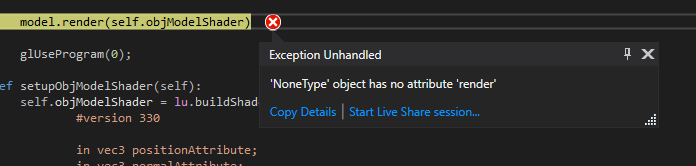
\includegraphics[width=0.8\textwidth, frame]
            {./images/mega_racer/1.3_a.PNG}
        \caption{1.3 -Error}
    \end{figure}

\textbf{(2) Loading the model}: 
In mega\_racer.py, \textit{g\_racer.load()} is called with three parameters; the object file for the racer (.obj), the terrain (Terrain()) and the rendering system (RenderingSystem()). 
    \begin{lstlisting}
# mega_racer.py
g_racer.load("data/racer_02.obj", g_terrain, g_renderingSystem)
-->
# racer.py - Racer
def load(self, objModelName, terrain, renderingSystem):
        .....    
    \end{lstlisting}

The purpose of \textit{load()} is to create and load the racer model. According to the project notes, the racer should be loaded as an instance of the ObjModel class, which corresponds to the use of \textit{drawObjModel()} for rendering. To initialise an instance of ObjModel, as per the \_\_init\_\_(), the only requirement argument is the filename which is given as \textit{objModelName}. The terrain and position variables are already assigned using the other parameters. Now the model for the racer has replaced the red dot and the movement of the racer is accurate.
    \begin{lstlisting}
    # racer.py - Racer
    def load(self, objModelName, terrain, renderingSystem):
            ..... 
        self.model = ObjModel(objModelName)
    \end{lstlisting}   

\begin{figure} [H]
    \centering
    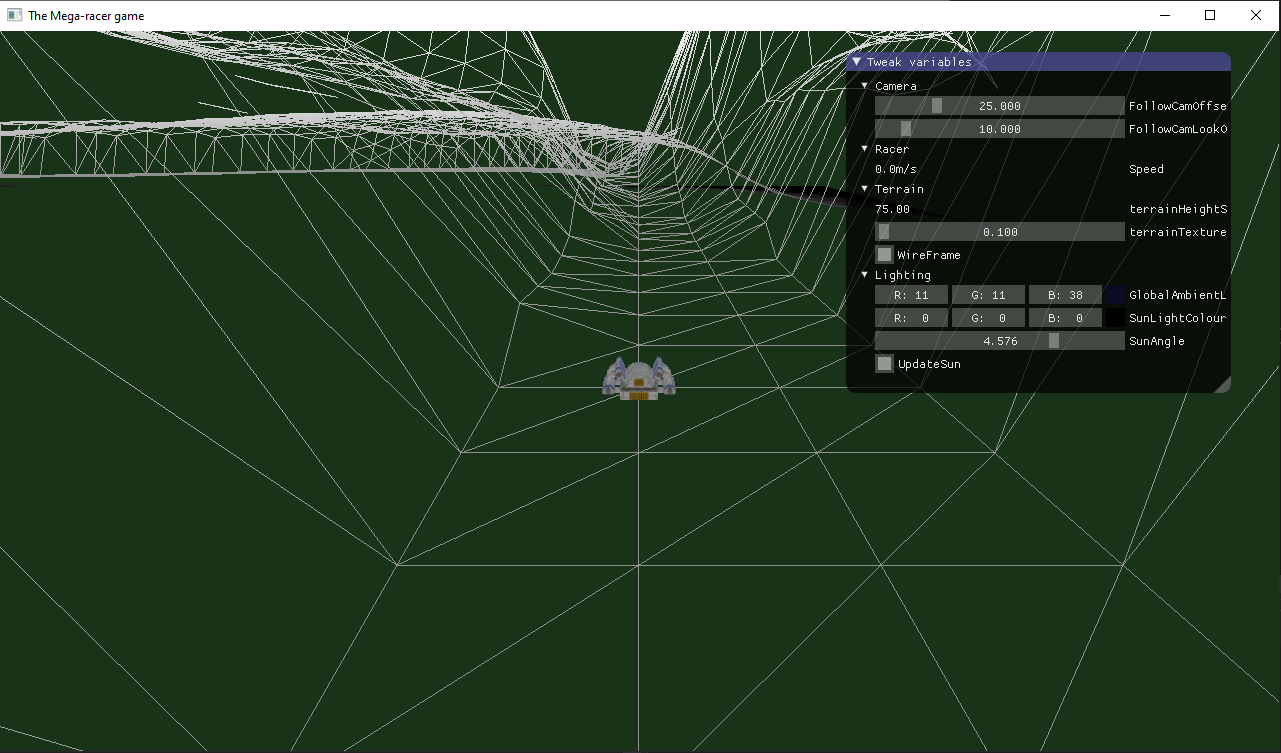
\includegraphics[width=0.8\textwidth, frame]
        {./images/mega_racer/1.3_b.PNG}
    \caption{1.3 - Final}
\end{figure}

%% 1.4
\subsubsection{1.4 - Texture the terrain}
Textures are a cheap and simple way to add detail that could not otherwise be provided simply by geometric modelling. Texture mapping is simply 'gluing images to surfaces' [47]. In this task a grass texture will be added over the whole world using 2D texturing. To repeat the texture every metre tiling (texture repetition) will be used to continuously repeat the image to avoid loss of resolution. There are three steps to complete this section in terrain.py. 

\textbf{(1) render() - Bind the grass texture to the right texture unit.} \\ 
In order to bind the texture, the hint is to is to use lu.bindTexture. This function, bindTexture(), takes two arguments texUnit and textureId. A similar function, with the same name, is used specifically in lab 5 question 12 [50]. Additionally, setUniform() needs to be called to prepare the texture for the shader. 
    \begin{lstlisting}
# Lab - lab_utils.py 
def bindTexture(texUnit, textureId, textureType = GL_TEXTURE_2D):
    ...
    -->
# Lab 5 Q12 - lab_5_template_2.py
g_detailTexture = None
def renderFrame(...):
    .....
    lu.bindTexture(0, g_detailTexture)
    lu.setUniform(g_shaderProgram, "baseTexture", 0)
    \end{lstlisting}

Following the same process, both \textit{bindTexture()} and \textit{setUniform} require the values of the texture unit allocation and the id of the texture. The \textit{textUnit} for grass is already assigned as \textit{TU\_Grass} = 0 in terrain.py. The \textit{textureId} was then declared within Terrain as \textit{grassTexture} equal to None. Additionally, setUniform() requires a shader to be passed, which is already declared as \textit{shader}, and a string name for the texture. In this case the same name as the texture id is used to minimise confusion. With these values declared, the two functions are called in the same way in \textit{render()}.
    \begin{lstlisting} 
# terrain.py
grassTexture = None

def render(...):
    ....
    lu.bindTexture(self.TU_Grass, self.grassTexture)
    lu.setUniform(self.shader, "grassTexture", self.TU_Grass)        
    \end{lstlisting}

\textbf{(2) load(): Compute the texture coordinates and sample the texture for the grass and use as material colour.} \\
As per the project notes the variable textureXyScale is to be used to scale the texture coordinates and is already set to a factor of 0.1 so the texture repeats every 10 metres. Also the world space coordinates should be used to sample the texture in the fragment shader. To determine how to set the sample, question 12 from lab 5 [50] provided insight into how to set the texture as the colour in the fragment shader.
\begin{lstlisting}
# Lab 5 - Q12  
g_texCoordScale = 7.0
def renderFrame():
    ...
    lu.setUniform(g_shaderProgram, "detailTexture", 1)
    lu.setUniform(g_shaderProgram, "texCoordScale", g_texCoordScale)
    ...
def initResources():
    .....         
    in vec2 v2f_textureCoord;
    uniform sampler2D detailTexture; 
    uniform float texCoordScale; 
    out vec4 fragmentColor;
    void main() 
    {   ...     
        vec3 detailColour = texture(detailTexture, 
                            v2f_textureCoord * texCoordScale).xyz;      
        ...
    }   
   
-->
# terrain.py
textureXyScale = 0.1
def load():
    ...
    lu.setUniform(self.shader, "terrainTextureXyScale", self.textureXyScale);
    ...
    fragmentShader = 
    ...
        uniform float terrainTextureXyScale;
        out vec4 fragmentColor;
        void main()
        {
            vec3 materialColour = vec3(v2f_height/terrainHeightScale);
            ...
        }
\end{lstlisting}

From this example it is evident that for the materialColour (i.e. detailColour) to reflect the texture it needs to be assigned the output of texture() with the following three arguments:
    \begin{itemize}
        \item detailTexture: The grass colour is similar to the detailColour so the detailTexture is equivalent to the grassTexture.
        \item v2f\_textureCoord: In lab 5 [50] the v2f\_textureCoord is a 2 dimensional out vector from the vertex shader. It refers to the location in texture space. As per the project notes, since the vertex is regular, this same behaviour can be replicated by only selecting the x and y coordinates of the world space which are stored in v2f\_worldSpacePosition.
        \item texCoordScale: The textCoordScale variable in lab 5 [50] refers to \textit{g\_texCoordScale} in mega racer which is declared and uniformly set for the shader as texCoordScale. The same is done for textureXyScale in Terrain which as mentioned is nominated in the project notes as the scale for the texture coordinates.
    \end{itemize}

Putting this all together, the texture coordinates were calculated and the texture of the grass was sampled to override the existing material colour.
    \begin{lstlisting}
# terrain.py - Terrain
def load(...):
    ...
    fragmentShader =
        ...
        uniform sampler2D grassTexture; 
        void main()
        {
            vec3 grassColour = texture(grassTexture, 
                                        v2f_worldSpacePosition.xy 
                                            * terrainTextureXyScale).xyz;
            materialColour = grassColour;
            ...
        }
    \end{lstlisting}

\textbf{(3) load() - fragmentShader: Load texture and configure the sampler.} \\
Also in lab 5 [50], in initResources() after declaring the shader the image is opened and the texture is mapped (glTextParameter), then the texture is loaded using lu.loadTexture(). A similar function can be found in the ObjModel.py (instead of lab\_utils.py) and performs the same actions. It also sets the texture to wrap repeatedly as desired.
    \begin{lstlisting}  
# Lab 5 
g_detailTexture = lu.loadTexture("data/details.jpg");
--> 
def loadTexture(fileName): 
    ....

# ObjModel.py - ObjModel
def loadTexture(self, fileName, basePath, srgb):
    ......
    glTexParameteri(GL_TEXTURE_2D, GL_TEXTURE_WRAP_S, GL_REPEAT);
    glTexParameteri(GL_TEXTURE_2D, GL_TEXTURE_WRAP_T, GL_REPEAT);
    \end{lstlisting}

To load the texture for the terrain this function needs to be called with the relevant parameters. The \textit{fileName} refers to the name of grass images and the srgb refers to whether it is a 2D image. Using this method the grass is generated with scalability, repetition and compression (Lecture 6).
    \begin{lstlisting}  
# terrain.py - Terrain
def load(...):
    self.grassTexture = ObjModel.loadTexture("grass2.png", "data", True)
    \end{lstlisting}

\begin{figure} [H]
    \centering
    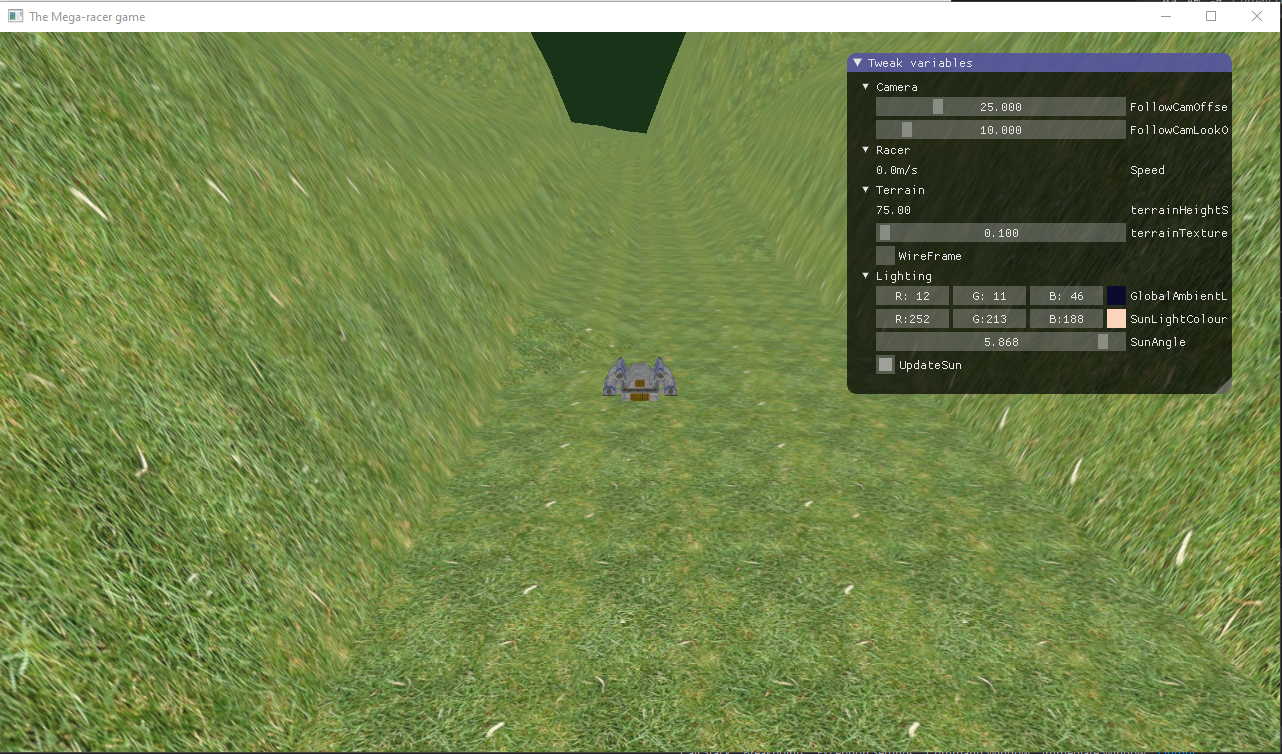
\includegraphics[width=0.8\textwidth, frame]
        {./images/mega_racer/1.4.PNG}
    \caption{1.4 - Final}
\end{figure}


% 1.5
\subsubsection{1.5 Lighting from the sun}  
Lighting provides a more realistic touch and assists with showing the structure of surfaces. Since this is light from the sun, this is a directional light and it can be assumed that the light rays are parallel since the light source is infinitely far away. A couple of things to note about this source of light:
\begin{itemize}
    \item Position of sun = g\_sunPosition: The sun is set to move around around the world.
    \item Colour of sunlight = g\_sunLightColour = lightColour
    \item Sun is defined in world space
\end{itemize}

The project notes explain that the code for the light should be added to the computeShading() function in RenderingSystem class as part of the commonFragmentShaderCode variable. This function is called in setUpModelShader() where the viewSpaceNormal and viewSpacePosition variables are declared by the vertex shader, materialColour is declared as materialDiffuse in the fragment shader, and viewSpaceLightPosition and sunLightColour are carried over from the commonShaderCode variable. 
    \begin{lstlisting}
#  mega_racer.py - RenderingSystem
def setupObjModelShader(...):
    v2f_viewSpaceNormal = normalize(modelToViewNormalTransform * normalAttribute);
    v2f_viewSpacePosition = (modelToViewTransform 
                                * vec4(positionAttribute, 1.0)).xyz;
    .....
    vec3 materialDiffuse = texture(diffuse_texture, 
                                    v2f_texCoord).xyz 
                                    * material_diffuse_color;
    vec3 reflectedLight = computeShading(materialDiffuse, 
                                            v2f_viewSpacePosition, 
                                            v2f_viewSpaceNormal, 
                                            viewSpaceLightPosition, 
                                            sunLightColour
                                        ) + material_emissive_color;
    \end{lstlisting}

When computing the light, the following tips must be adhered to:
    \begin{itemize}     
        \item All parameters om shading must be the same space -> set as view space (same as lab 4 [50])         
        \item The computeShading function needs to be called from each function -> this is already done.
        \item Need to make sure don't just have Lambertian term -> Fixed by multiplying by materialDiffuse term.
        \item Use clamping to check when light is behind surface.
    \end{itemize}

To create the lighting effect required, all of the code followed that of fragmentShader.glsl in Lab 4 [50]. Question 1 was already provided as a basic shader. The view space is used for shading calculations. The computeShading() function is setup with five parameters, all of which are used to return a light value.
    \begin{lstlisting}
# mega_racer.py - RenderingSystem
commonFragmentShaderCode =
    ...
    vec3 computeShading(vec3 materialColour, 
                        vec3 viewSpacePosition, 
                        vec3 viewSpaceNormal, 
                        vec3 viewSpaceLightPos, 
                        vec3 lightColour)
    {
        return lightValue;
    }
    \end{lstlisting}

\textbf{(1) The direction towards the source of the light.} \\
Starting from Lab 4 [50], question 2, the first step was to compute the normalised direction towards the light from the shading point in view space. The light position is stored as viewSpaceLightPosition and the current point is viewSpacePosition (provided by the vertex shader). 
    \begin{lstlisting}
# Lab 4 - Q2 - FragmentShader
vec3 viewSpaceDirToLight = normalize(viewSpaceLightPosition - viewSpacePosition);
    
# mega_racer.py - RenderingSystem
commonFragmentShaderCode =
    ...
    vec3 computeShading(...)
    {
        vec3 viewSpaceDirToLight = normalize(viewSpaceLightPos- viewSpacePosition);
        return viewSpaceDirToLight;
    }
    \end{lstlisting}

    \begin{figure} [H]
        \centering
        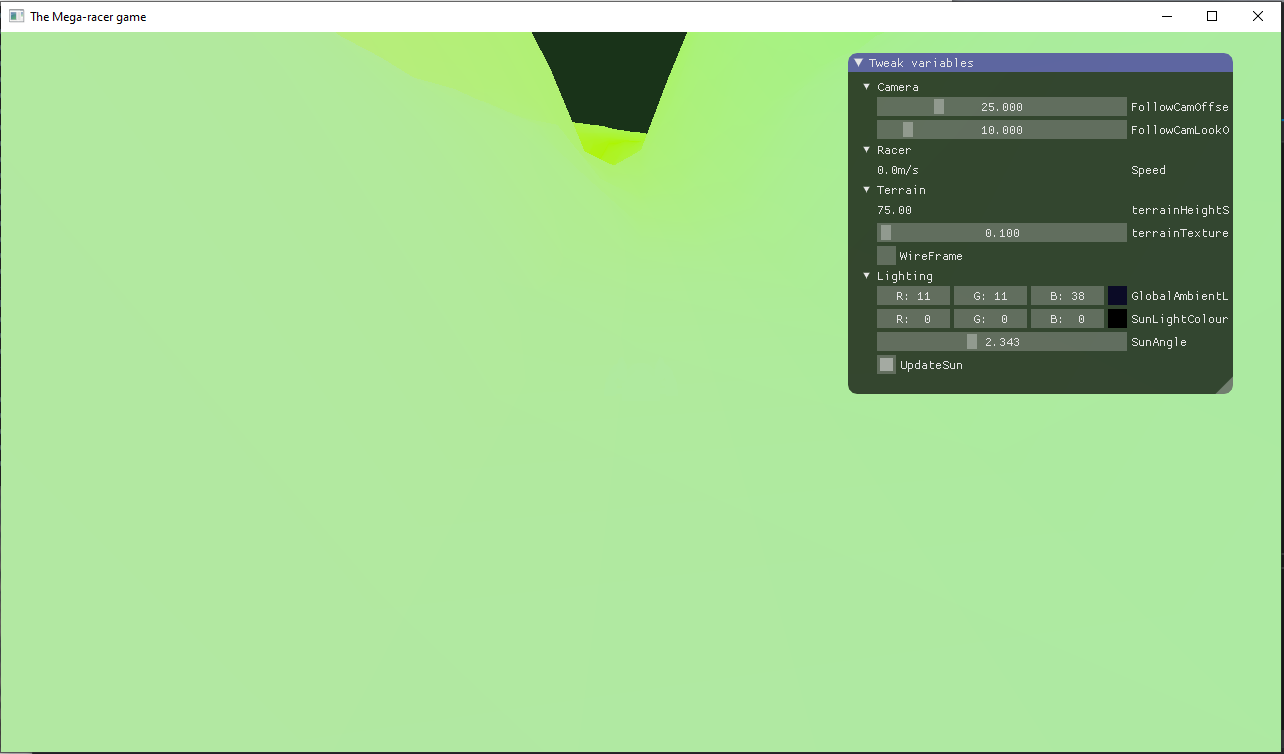
\includegraphics[width=0.8\textwidth, frame]
            {./images/mega_racer/1.5_a.PNG}
        \caption{1.5 - Step 1}
    \end{figure}

\textbf{(2) Compute the incoming light intensity.}
Using the now defined \textit{viewSpaceDirToLight}, the incoming light intensity can be calculated. As mentioned, in mega\_racer.py three variable of viewSpaceNormal is already provided by the vertex shader. This maintains the unit-length property of the normal.
    \begin{lstlisting}
# Lab 4 - Q2 - FragmentShader
vec3 viewSpaceNormal = normalize(v2f_viewSpaceNormal);
float incomingIntensity = max(0.0, dot(viewSpaceNormal, viewSpaceDirToLight));

# mega_racer.py - RenderingSystem
commonFragmentShaderCode =
    ...
    vec3 computeShading(...)
    {
        ...
        float incomingIntensity = max(0.0, dot(viewSpaceNormal, viewSpaceDirToLight));
        return incomingIntensity;
    }
    \end{lstlisting}

    \begin{figure} [H]
        \centering
        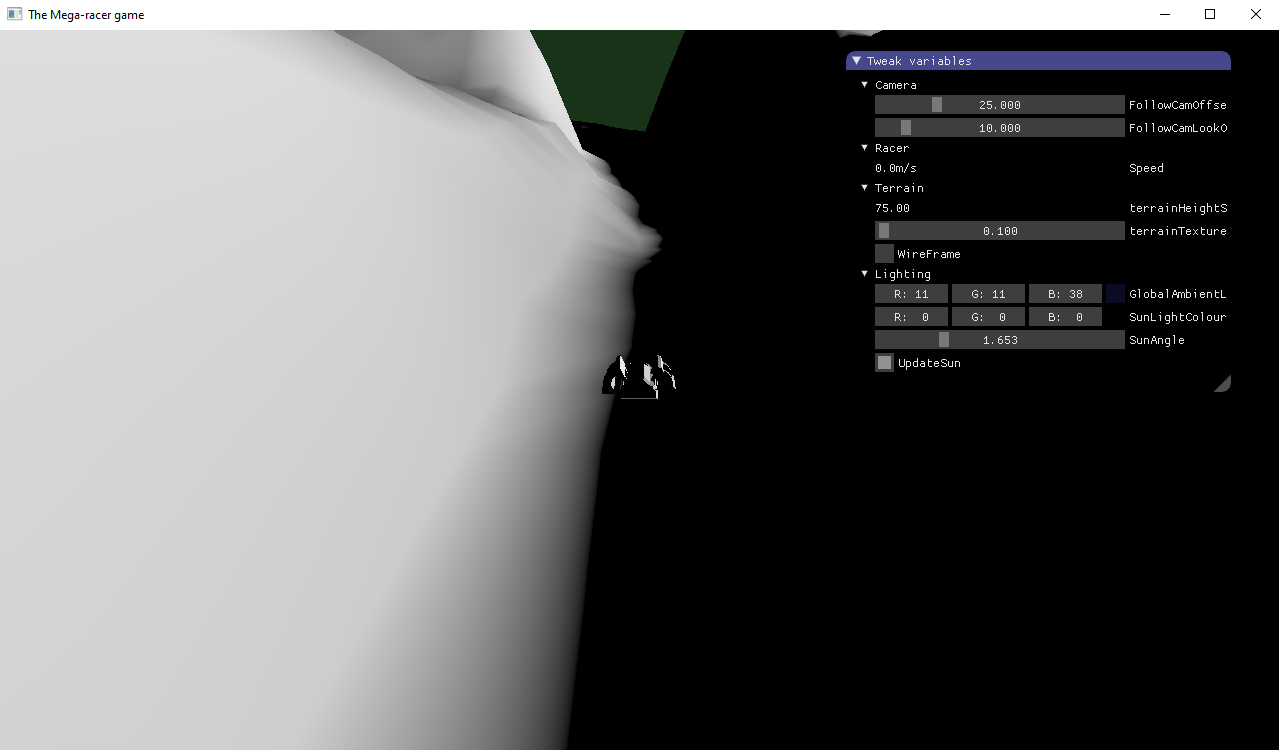
\includegraphics[width=0.8\textwidth, frame]
            {./images/mega_racer/1.5_b.PNG}
        \caption{1.5 - Step 2}
    \end{figure}


\textbf{(3) Modify the light that is emitted by the light source to have the correct colour and maximum intensity.}
The distribution of incoming light that is arriving at the surface needs to be handled so the correct colour and maximum intensity are shown.
    \begin{lstlisting}
# Lab 4 - Q2 - FragmentShader
vec3 incomingLight = incomingIntensity * lightColourAndIntensity;

# mega_racer.py - RenderingSystem
commonFragmentShaderCode =
    ...
    vec3 computeShading(...)
    {
        ...
        vec3 incomingLight = incomingIntensity * lightColour;
        return incomingLight;
    }        
    \end{lstlisting}

    \begin{figure} [H]
        \centering
        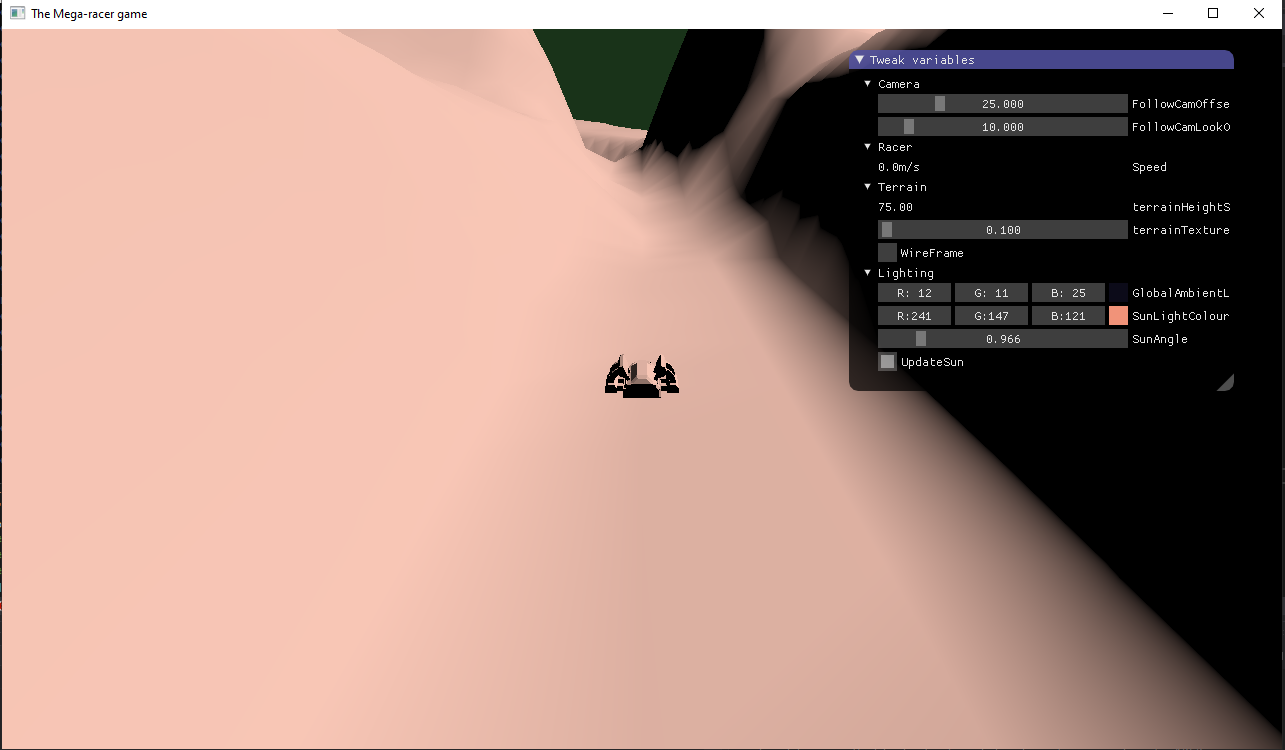
\includegraphics[width=0.8\textwidth, frame]
            {./images/mega_racer/1.5_c.PNG}
        \caption{1.5 - Step 3}
    \end{figure}
    
\textbf{(4) Diffuse Lambertian Reflection.}
The bidirectional reflection distribution (BRDF) is used widely to model how surfaces reflect light [46]. To diffuse the Lambertian reflection by multiplying the incoming light with a constant that represents the reflection of the material for the given spectrum. Following the same pattern as question 3 in lab 4 [50], the argument passed as materialColour should provide this representation, as provided by the materialDiffuse variable passed in to computeShading() in setUpObModelShader(). 
    \begin{lstlisting} 
# Lab 4  - FragmentShader
vec3 materialDiffuse = texture(diffuse_texture, v2f_texCoord).xyz 
                                * material_diffuse_color;
vec3 outgoingLight = incomingLight * materialDiffuse;

# mega_racer.py - RenderingSystem
commonFragmentShaderCode =
    ...
    vec3 computeShading(...)
    {
        ...
        vec3 outgoingLight = incomingLight * materialColour;
        return outgoingLight;
    }                            
    \end{lstlisting}

    \begin{figure} [H]
        \makebox[\textwidth]{%
        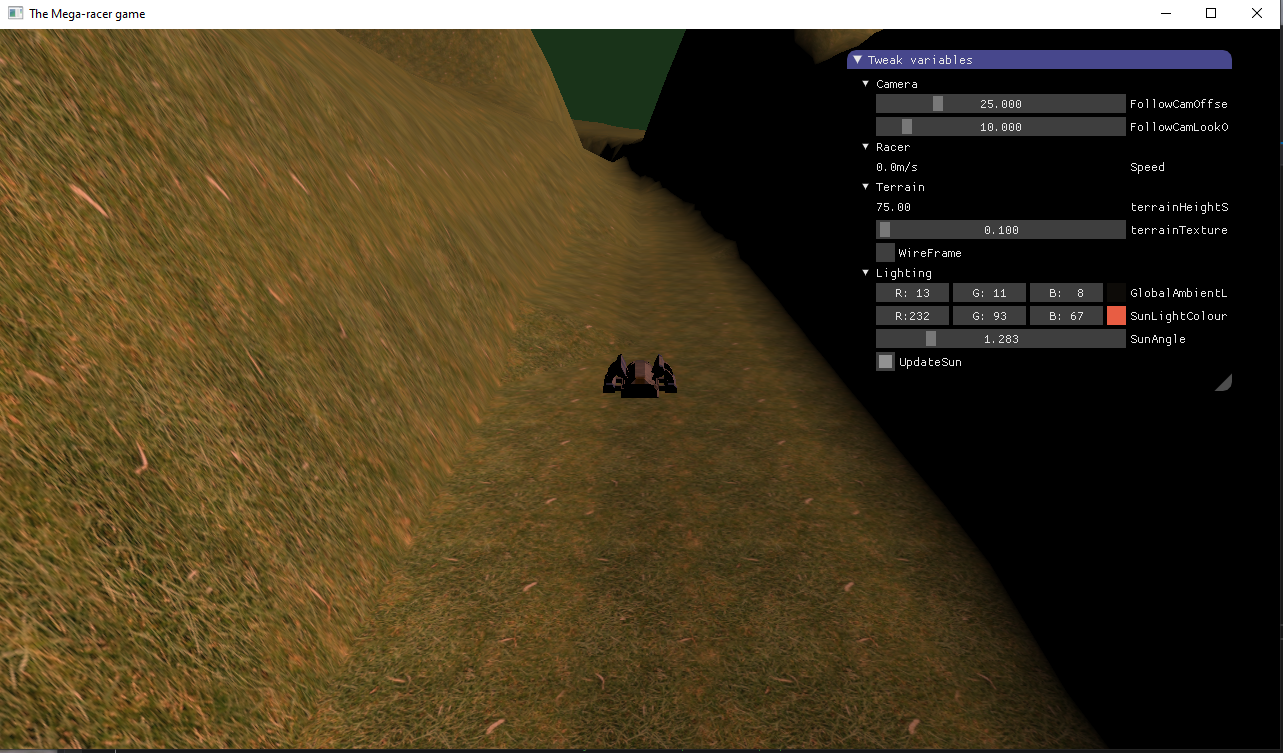
\includegraphics[width=0.49\textwidth, frame]
            {./images/mega_racer/1.5_d_1.PNG}%
        \hfill
        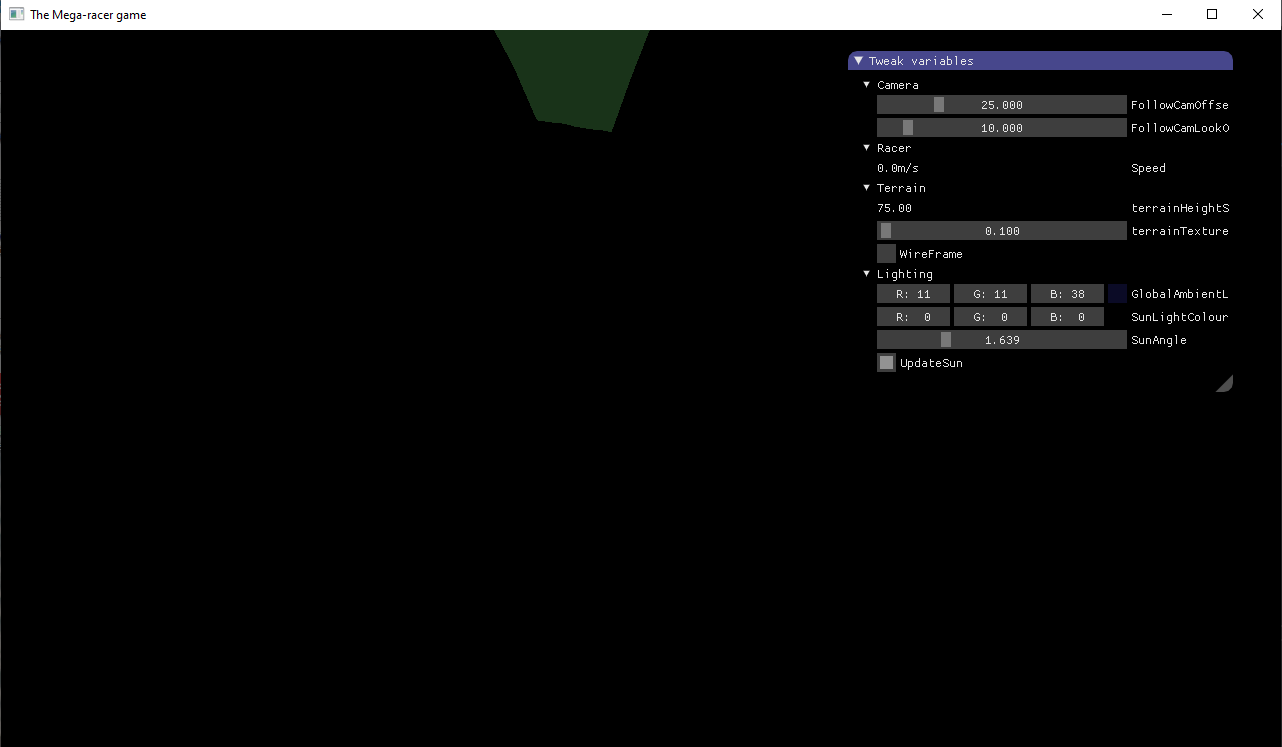
\includegraphics[width=0.49\textwidth, frame]
            {./images/mega_racer/1.5_d_2.PNG}
        }        
        \caption{1.5 - Step 4}   
    \end{figure}

\textbf{(5) Take into account the indirect light.}
In order to handle indirect lighting, it is replaced by a constant that is known as ambient lighting. This step builds on step 3 and follows question 4 in lab 4 [50]. As mentioned in the notes, this is an approximation with a single colour value. The ambience is added to the incomingLight variable as there is the light comes from everywhere, and then multiplied by the BRDF as both are independent.
    \begin{lstlisting}[language=c++] 
# Lab 4  - FragmentShader
vec3 outgoingLight = (incomingLight + ambientLightColourAndIntensity) 
                        * materialDiffuse;

# mega_racer.py - RenderingSystem
commonFragmentShaderCode =
    ...
    vec3 computeShading(...)
    {
        ...
        vec3 outgoingLight = (incomingLight + globalAmbientLight) 
                            * materialColour;
        return outgoingLight;
    }       
    \end{lstlisting}

This has produced the final results, light that doesn't cause pitch black and reflects according to the correct colour.
    \begin{figure} [H]
        \makebox[\textwidth]{%
        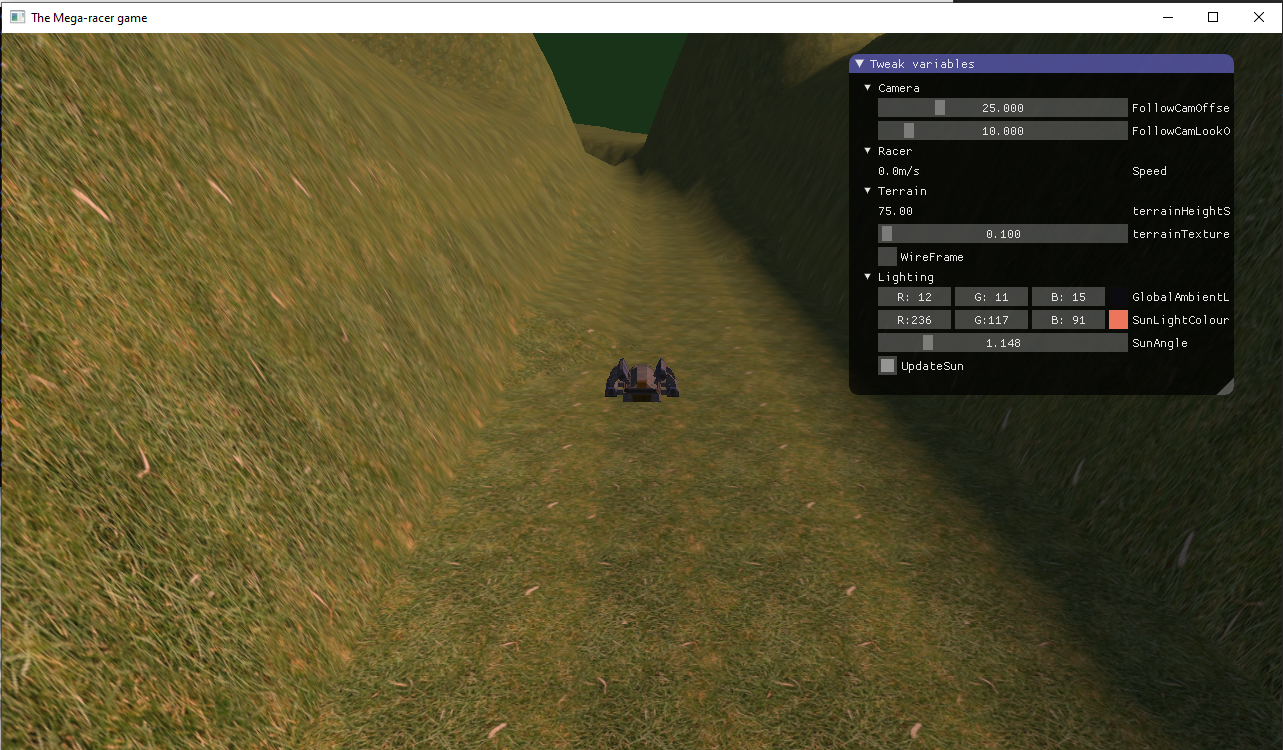
\includegraphics[width=0.49\textwidth, frame]
            {./images/mega_racer/1.5_e_1.PNG}%
        \hfill
        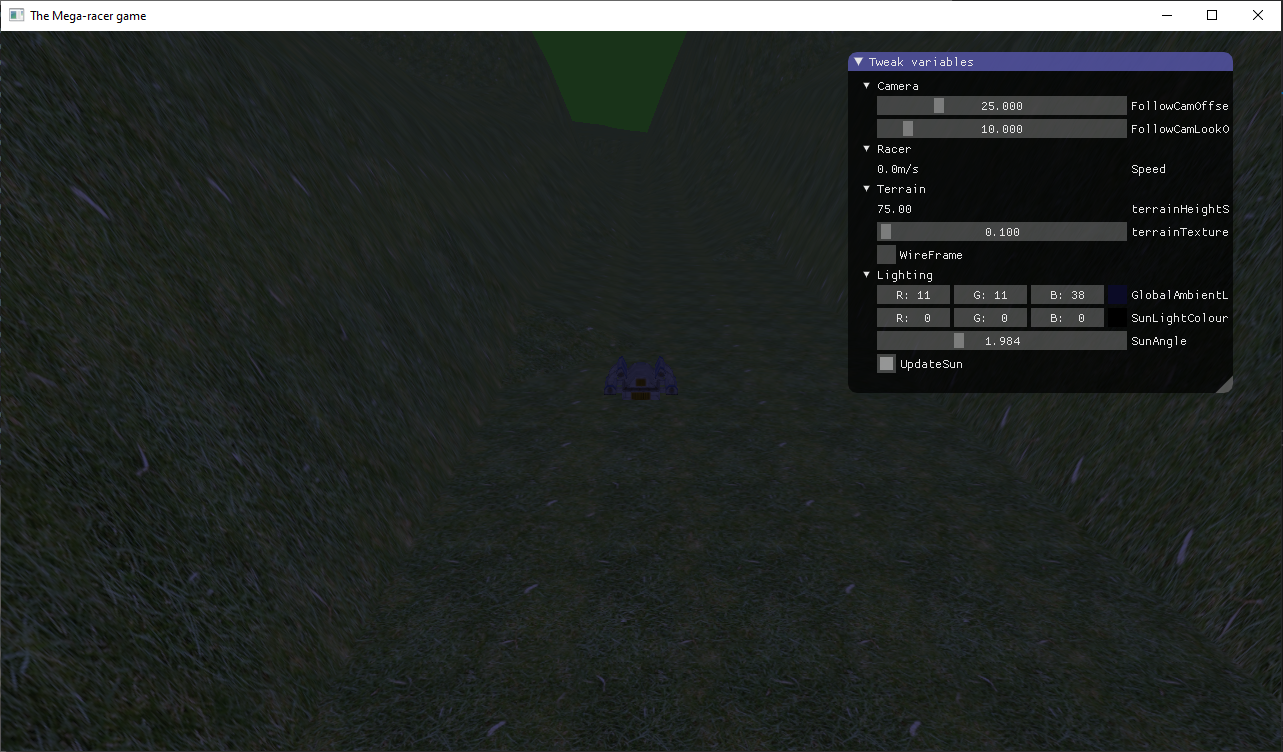
\includegraphics[width=0.49\textwidth, frame]
            {./images/mega_racer/1.5_e_2.PNG}
        }
        
        \caption{1.5 - Step 5}   
    \end{figure}

\textbf{Side notes:} There are many other lighting models that could have been introduced; including a more advanced ambient model or specular lighting. 


%%%% TIER 2 %%%%%%%
\subsection{Tier 2}
The following deliverables were a higher difficulty and required more time, effort and research to complete. The tasks that were chosen were to improve terrain textures, add fog and add props. These tasks were all completed to a good standard, though improvements can always be made. Additionally, these were all tasks that could be carried forward to the Olympic Stadium model. 

\subsubsection{2.1 Improve terrain textures}
Adding extra textures to the world not only offers visual appeal with more a more realistic environment but also provides functional ques to the user about the type of terrain they are driving on (rough or road). There are three additional textures to add in this section; high, steep and road. For each of the textures, the same process as the grassTexture was followed in terms of the following:
\begin{enumerate}
    \item Declare a texUnit and a texID to introduce the texture.
    \item Call bindTexture and setUniform to prepare it for the shader.
    \item Assign the texture as the \textit{materialColour} in the fragmentShader depending on height/slope logic.
    \item Load the texture with the matching 2D image.
\end{enumerate}


Both the highTexture and steepTexture are required to be mixed with the grassColour for a more realistic appearance. This function takes two vectors and weighting value between 0 and 1 (t), where the second vector argument is scalar multiplied by the t value and the first vector is multiplied by 1 minus the t value. Therefore more emphasis is placed on the second vector colour.
\begin{lstlisting}
def mix(v0, v1, t):
    return v0 * (1.0 - t) + v1 * t
\end{lstlisting}


\textbf{(1) Set the high texture}
The height texture should only be selected when the height in the world is above a certain threshold, as well as being mixed with the grass texture. The height is given by the vertex shader, which is the z position of the positionIn or worldSpacePosition variable. The terrainHeightScale is equivalent to Terrain.heightScale which is 75.0 and used as a scale factor to calculate the z coordinates for each vertex.
    \begin{lstlisting}
# vertexShader:
v2f_height = positionIn.z
    -> v2f_worldSpacePosition = positionIn 

# render
terrainHeightScale = self.heightScale 
    -> heightScale = 75.0
    \end{lstlisting}

The same steps as the grass texture are followed including declaring a unit, the texture variable, binding the texture, setting the uniform value and loading the texture. However, sampling the texture is slightly different as instead of overriding the materialColour with the highColour, the highColour is assigned in the same way at the given height and then the materialColour is assigned as the output of blending this highColour with the grassColour using mix().
\begin{lstlisting}
# terrain.py
TU_High = 1
highTexture = None

def render():
    ....
    lu.bindTexture(self.TU_High, self.highTexture)
    lu.setUniform(self.shader, "highTexture", self.TU_High)

def load():
    fragmentShader = 
        ...
        uniform sampler2D highTexture;

        void main():
        {   ....
            OR if (v2f_height > 50) {
            if ((v2f_height/terrainHeightScale) > 0.9) {
                vec3 highColour = texture(highTexture, 
                                    v2f_worldSpacePosition.xy 
                                    * terrainTextureXyScale).xyz;
                materialColour = mix(materialColour, 
                                    highColour, 
                                    (v2f_height/terrainHeightScale));
        } 
    
    self.highTexture = ObjModel.loadTexture("rock 2.png", "data", True)        
        \end{lstlisting}

    \begin{figure} [H]
        \centering
        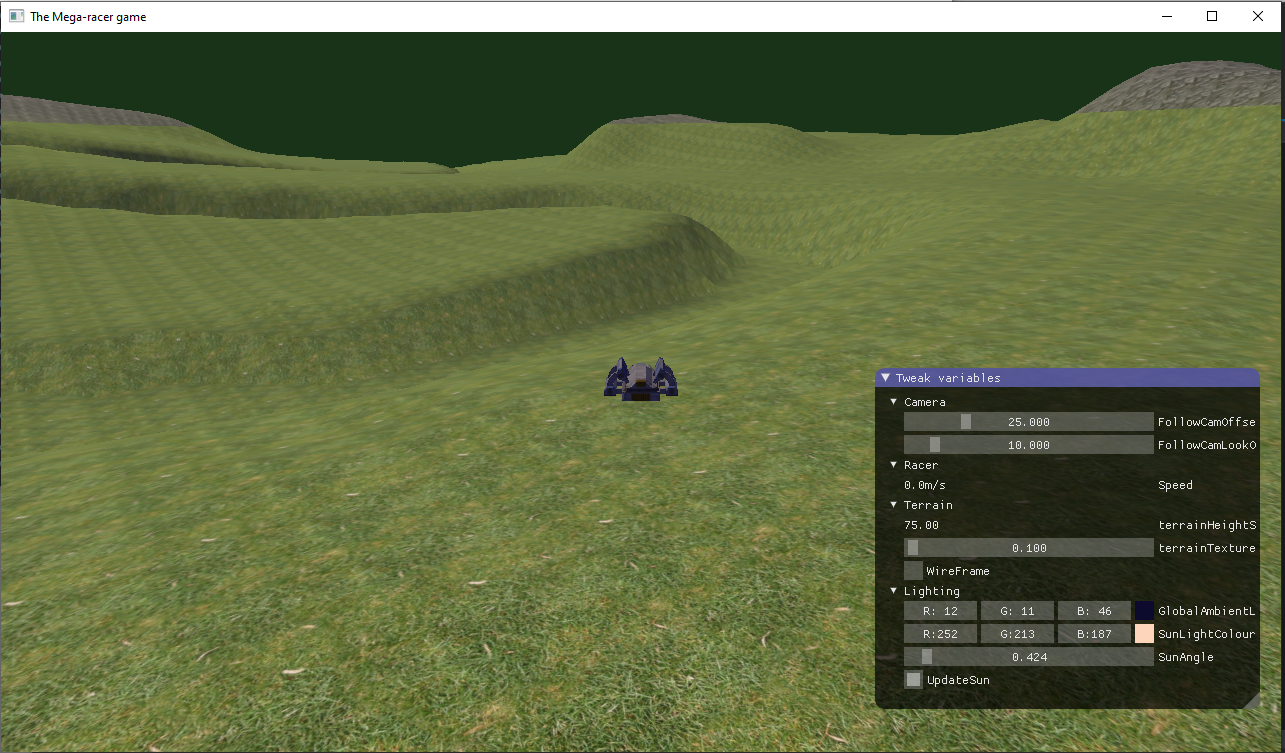
\includegraphics[width=0.8\textwidth, frame]
            {./images/mega_racer/2.1_a.PNG}
        \caption{2.1 - High Texture}   
    \end{figure}


\textbf{(2) Set the steep texture}
The steep texture relies on only be loaded when the slope meets a certain threshold. To get the slope, first the coordinates of the normalised world space need to be available. The viewSpacePosition, viewSpaceNormal and worldSpacePosition had already been provided, and so the same pattern was followed to have access to the worldSpaceNormal.
    \begin{lstlisting}
vertexShader =
    out VertexData
    {
        vec3 v2f_viewSpacePosition;
        vec3 v2f_viewSpaceNormal;
        vec3 v2f_worldSpacePosition;
        vec3 v2f_worldSpaceNormal; // NEW
    }
    void main()
    {
        v2f_viewSpacePosition = (modelToViewTransform * vec4(positionIn, 1.0)).xyz;
        v2f_viewSpaceNormal = modelToViewNormalTransform * normalIn;
        v2f_worldSpacePosition = positionIn;
        v2f_worldSpaceNormal = normalIn; // NEW
    }
fragmentShader = 
    in VertexData
    {
        vec3 v2f_viewSpacePosition;
        vec3 v2f_viewSpaceNormal;
        vec3 v2f_worldSpacePosition;
        vec3 v2f_worldSpaceNormal; // NEW
    }
    \end{lstlisting}

Now that the normalised world space is available to use, the slope needs to be calculated and compared to the threshold to determine when to blend the textures. Again, the same steps are followed to map the texture, however the slope is calculated and then the logic of the threshold applied. 
    \begin{lstlisting}
# terrain.py
TU_Steep = 2
steepTexture = None

def render():
    ....
    lu.bindTexture(self.TU_Steep, self.steepTexture)
    lu.setUniform(self.shader, "steepTexture", self.TU_Steep)

def load():
    fragmentShader = """
        ...
        uniform sampler2D steepTexture;

        void main()
        {....
            float slope = dot(v2f_worldSpaceNormal, vec3(v2f_worldSpaceNormal.x, 
                                                            0.0, 
                                                            v2f_worldSpaceNormal.z));
            if (slope < 0.8) {
                vec3 steepColour = texture(steepTexture, 
                                    v2f_worldSpacePosition.xy 
                                        * terrainTextureXyScale).xyz;
                materialColour = mix(materialColour, steepColour, 
                                    (v2f_height/terrainHeightScale));
        } 

    self.steepTexture = ObjModel.loadTexture("rock 5.png", "data", True)
    \end{lstlisting}

    \begin{figure} [H]
        \centering
        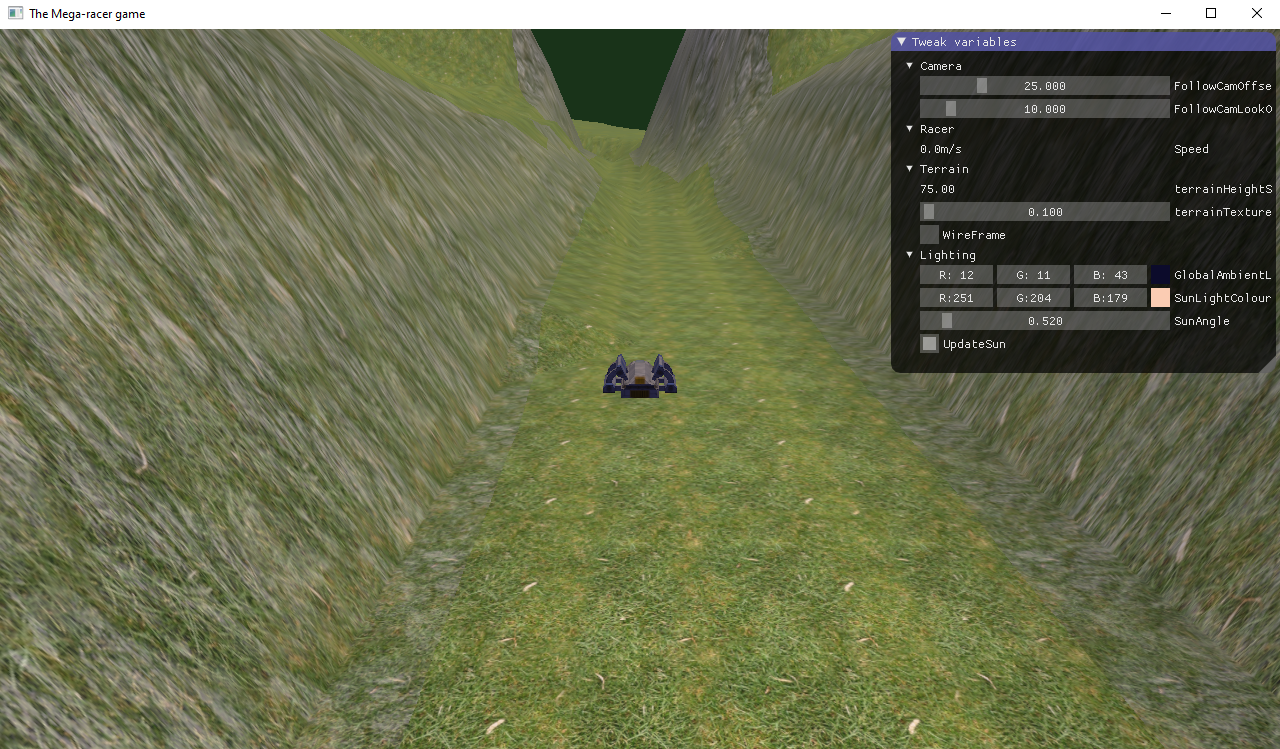
\includegraphics[width=0.8\textwidth, frame]
            {./images/mega_racer/2.1_b.PNG}
        \caption{2.1 - Steep Texture}   
    \end{figure}


\textbf{(3) Add the road}
To load a texture for the road, since the game logic is not available to the fragment shader, a mapTexture needed to be created which could identify the \textit{blueChannel} of the map for the shader. As previously mentioned, the blue pixel on the map is used to represent the road and subsequently the logic of the racer's speed. Since the track image is not a 2D file, when calling ObjModel.loadTexture the SRGB parameter is passed is False. As well as creating this map texture, a road texture also needs to be created, following the same steps as the grass texture. However, the logic in the fragmentShader was quite different and will be explained separately.

\begin{lstlisting}
# terrain.py
TU_Road = 3
TU_Map = 4
roadTexture = None
mapTexture = None

def render():
    ....
    lu.bindTexture(self.TU_Road, self.roadTexture)
    lu.bindTexture(self.TU_Map, self.roadMap)
    lu.setUniform(self.shader, "roadTexture", self.TU_Road)
    lu.setUniform(self.shader, "mapTexture", self.TU_Map)

def load():
    fragmentShader = 
        ...
        uniform sampler2D roadTexture;
        uniform sampler2D mapTexture;

        void main():
        {   ....
            ????
        }
        }
    
    self.roadTexture = ObjModel.loadTexture("paving 5.png", "data", True)
    self.mapTexture = ObjModel.loadTexture("track_01_128.png", "data", False)
\end{lstlisting}

For the high and steep textures, the shader was relying simply on the height and slope, but now to for the shader to know what is considered 'road' the blueChannel needs to be calculated using the mapTexture. To be able to sample this texture the first step was to get the normalised texture coordinates. This was possible by following the similar steps to the worldSpaceNormal but with the xyNormScale and xyOffset. These were the last two declared variables in the vertex shader that hadn't been carried through to the fragment shader despite being declared as uniform in render() at the same time as the Texture XyScale and HeightScale. It was obvious that the xyNormScale variable would be used instead of terrainTextureXyScale, but the purpose of the offset was unclear at this time. 
    \begin{lstlisting}
# render()      
xyNormScale = 1.0 / (vec2(self.imageWidth, self.imageHeight) * self.xyScale);
lu.setUniform(self.shader, "xyNormScale", xyNormScale);
xyOffset = -(vec2(self.imageWidth, self.imageHeight) + vec2(1.0)) * self.xyScale / 2.0;
lu.setUniform(self.shader, "xyOffset", xyOffset);
--> 

# load()
vertexShader =
    out VertexData
    {
        vec2 v2f_xyNormScale;
        vec2 v2f_xyOffset;
    }
    void main()
    {
        v2f_xyNormScale = xyNormScale;
        v2f_xyOffset = xyOffset;
    }
fragmentShader = 
    in VertexData
    {
        vec2 v2f_xyNormScale;
        vec2 v2f_xyOffset;
    }
        \end{lstlisting}

When working on this section, it was often difficult to determine the problem, as unless the texture was declared, bound and loaded properly in the shader nothing would display. The below code is the first iteration that provided 'working' shading. The blueChannel variable followed that of the other textures, though instead of multiplying the worldSpacePosition.xy by the terrainTextureXyScale it was multiplied by the xyNormScale variable and only the z coordinate needed to be stored. The threshold of 0.9 was chosen as this produced the most accurate result. 
    \begin{lstlisting}
# terrain.py       
def load():
    fragmentShader =                 
        void main():
        {   ....
        float blueChannel = texture(mapTexture, v2f_worldSpacePosition.xy 
                                                    * v2f_xyNormScale).z;
        if (blueChannel >= 0.9) {
            vec3 roadColour = texture(roadTexture, v2f_worldSpacePosition.xy 
                                                    * terrainTextureXyScale).xyz;
            materialColour =  mix(materialColour, roadColour, 
                                    (v2f_height/terrainHeightScale));
            }
        }
    \end{lstlisting} 

\begin{figure} [H]
    \centering
    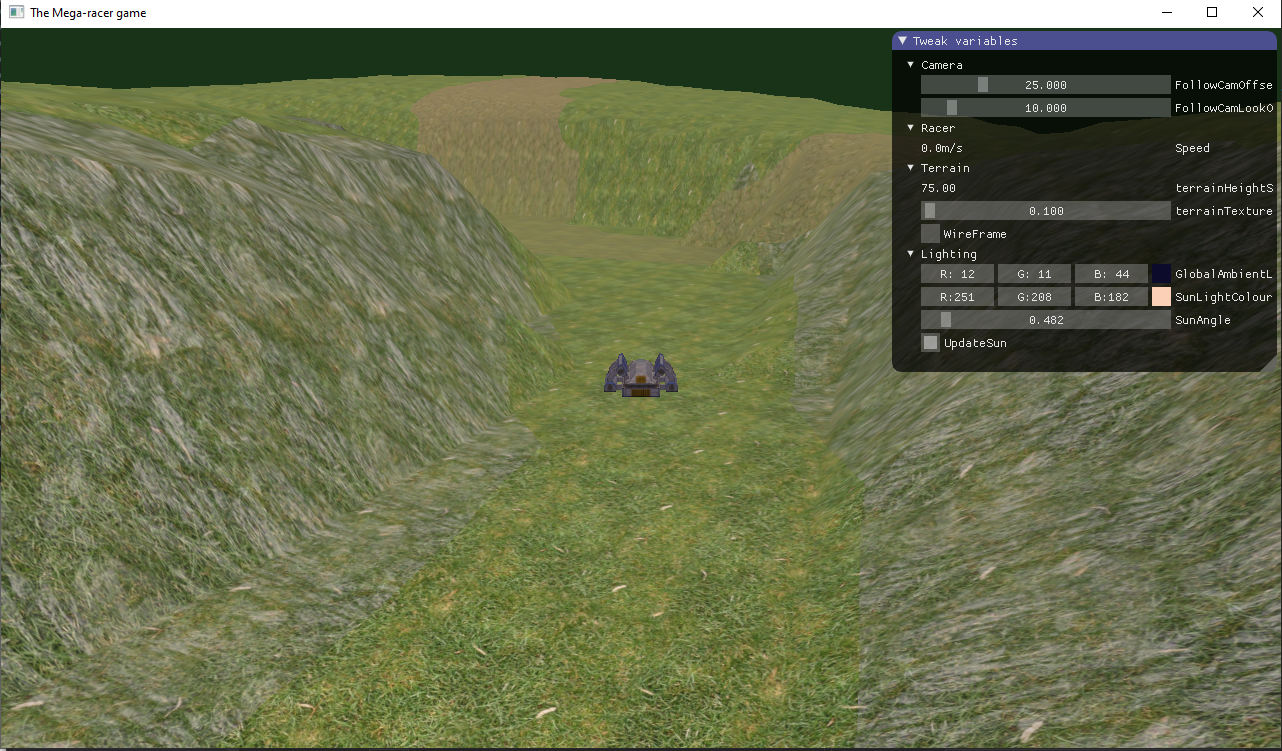
\includegraphics[width=0.8\textwidth, frame]
        {./images/mega_racer/2.1_c_1.PNG}
    \caption{2.1 - Road Texture (Mixed \& No Offset)}   
\end{figure}

There are clearly still some issues to resolve. 
\begin{enumerate}
    \item The grass texture was overtaking the blend of the pavement. This is because the roadColour was mixed with the grassColour as previously done. In the next iteration, the same as grassColour was followed such that only the roadColour would be declared as the materialColour when in the blueChannel.
    \item The road was not in the position it needed to be and was instead on the hill. This was another simple fixing by subtracting the xyOffset variable from the worldSpacePosition. After discovering this fixed the coordinates of the road, the mixing of road and grass was trialled again but the same issue occurred.
\end{enumerate}

\begin{figure} [H]
        \makebox[\textwidth]{%
        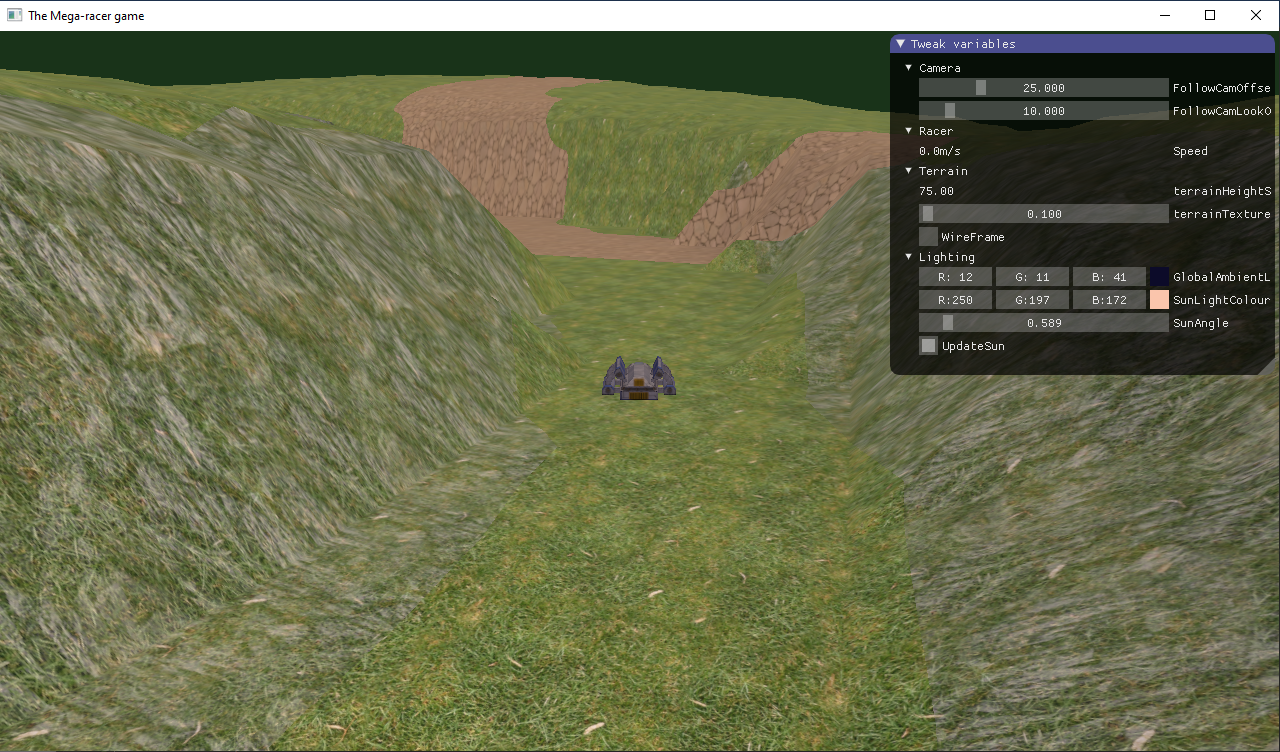
\includegraphics[width=0.49\textwidth, frame]
            {./images/mega_racer/2.1_c_2.PNG}%
        \hfill
        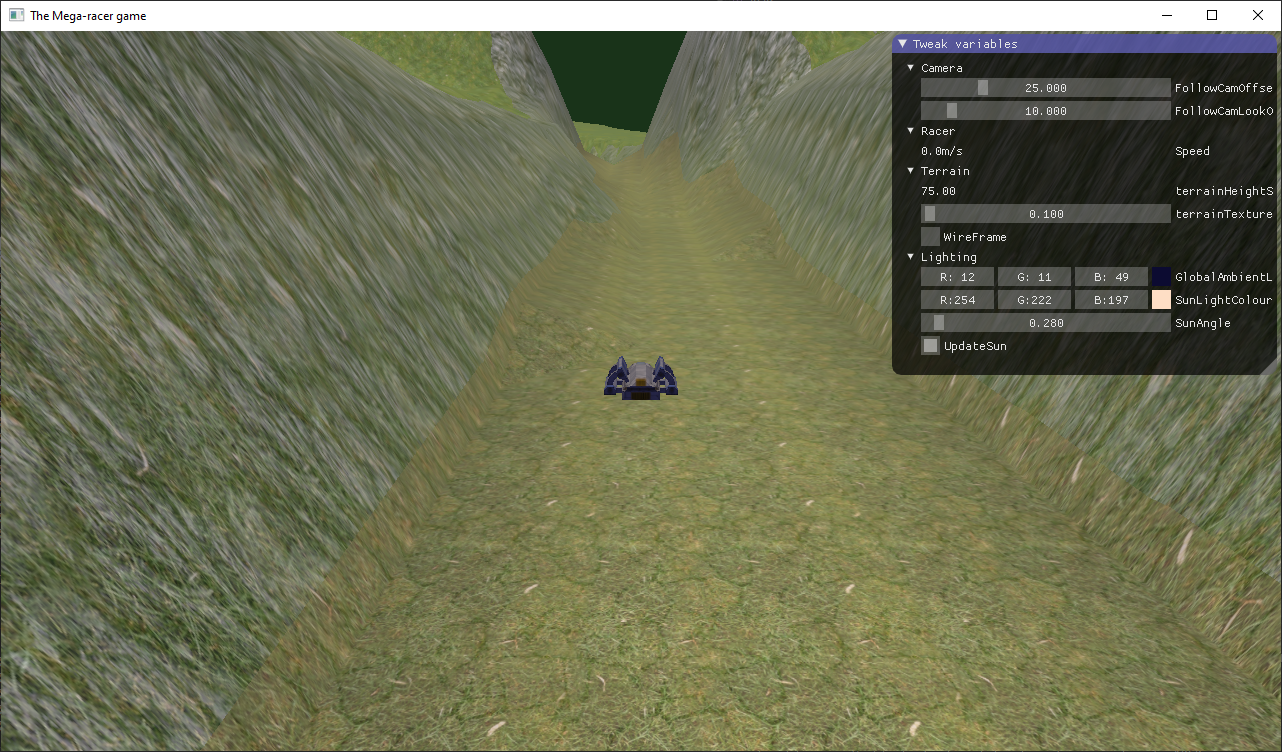
\includegraphics[width=0.49\textwidth, frame]
            {./images/mega_racer/2.1_c_3.PNG}        
        }        
        \caption{2.1 - Road Texture (Not Mixed \& No offset / Mixed \& Offset)}   
\end{figure}

After making these changes, the paving was successfully sampled and loading correctly onto the correct coordinates for the road according to the blue channel of the track.
    \begin{lstlisting}
# terrain.py       
float blueChannel = texture(mapTexture, 
                                (v2f_worldSpacePosition.xy - v2f_xyOffset) 
                                    * v2f_xyNormScale).z;
if (blueChannel >= 0.9) {
    vec3 roadColour = texture(roadTexture, 
                        v2f_worldSpacePosition.xy * terrainTextureXyScale).xyz;
        materialColour = roadColour;
}
    \end{lstlisting} 

    \begin{figure} [H]
        \centering
        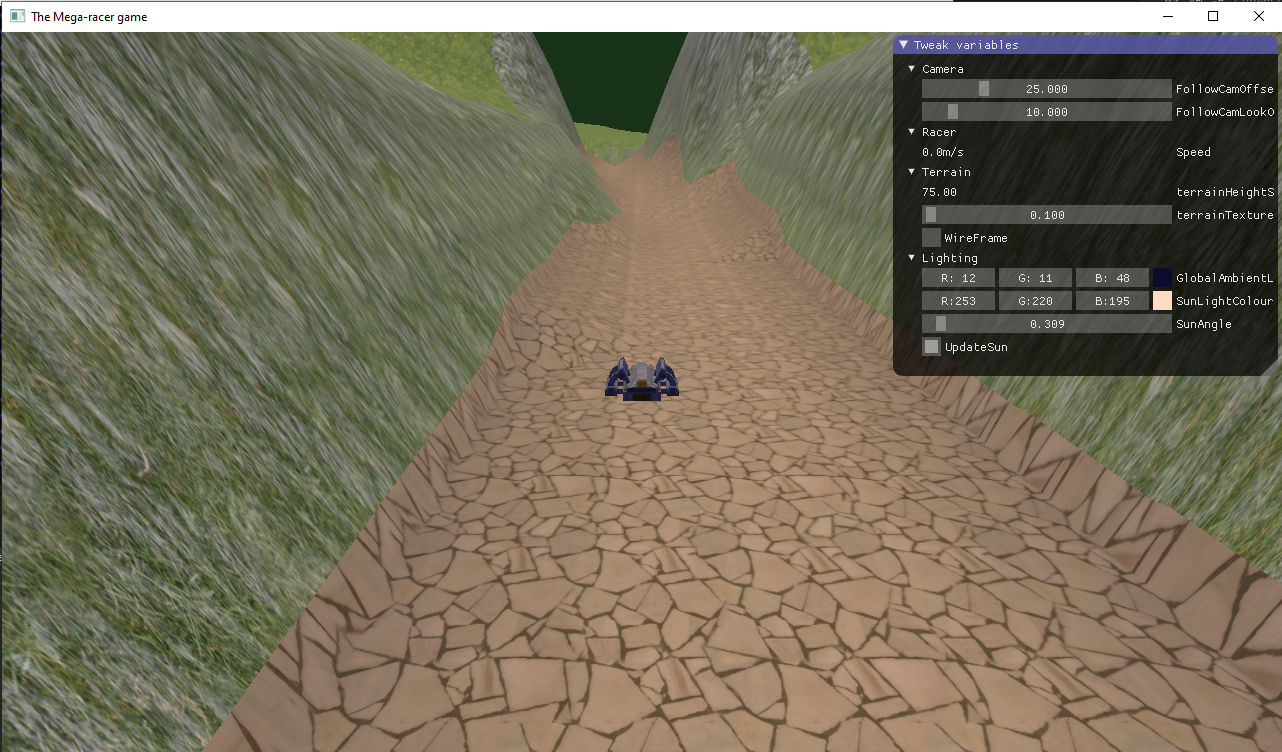
\includegraphics[width=0.8\textwidth, frame]
            {./images/mega_racer/2.1_c_final.PNG}
        \caption{2.1 - Road Texture}   
    \end{figure}


% 2.2 
\subsubsection{2.2 Add Fog}
Adding fog to the world was an attempt to provide the opportunity to add realism, depth, scaling of objects, give distance cues and more lighting effects to the world. The provided tutorial in the project notes was followed for this step to implement basic and then height-based fog.

\textbf{(1) Colour based fog)}
The first step of the tutorial was to implement colour to the fog, though it was referred to as scattering. This aimed to provide some context as to the strength of the sun by making the colour dependent on orientation. The b variable refers to the density and is set to 0.005 as per [3]. This function was declared in commonFragmentShaderCode in mega\_racer.py, then called as the output to fragmentColour in the fragmentShader. The relevant variables for the parameters are as follows:
    \begin{itemize}
        \item rgb = reflectedLight: This is currently the argument passed into toSrgb as for the 'color' parameter, so it will perform the same purpose as the 'rgb' parameter for applyFog().
        \item distance = -v2f\_viewSpacePosition.z \\      
        v2f\_viewSpacePosition = (modelToViewTransform * vec4(positionAttribute, 1.0)).xyz;
    \end{itemize}

    \begin{lstlisting}
# Tutorial
vec3 applyFog( in vec3  rgb, in float distance )
{
    float fogAmount = 1.0 - exp( -distance*b );
    vec3  fogColor  = vec3(0.5,0.6,0.7);
    return mix( rgb, fogColor, fogAmount );
}
-->
# mega_racer.py - Rendering system
commonFragmentShaderCode = 
    ...
    vec3 applyFog(in vec3 rgb, in float distance)
    {
        float b = 0.005;
        float fogAmount = 1.0 - exp(-distance*b);
        vec3  fogColor  = vec3(0.5,0.6,0.7);
        return mix(rgb, fogColor, fogAmount);
    }
#terrain.py
def load(...):
    ...
    fragmentShader = 
        ...
        void main()
        {
            ...
            fragmentColor = vec4(toSrgb(applyFog(reflectedLight, 
                                        -v2f_viewSpacePosition.z)), 1.0);
        }
    \end{lstlisting} 

\begin{figure} [H]
    \makebox[\textwidth]{%
    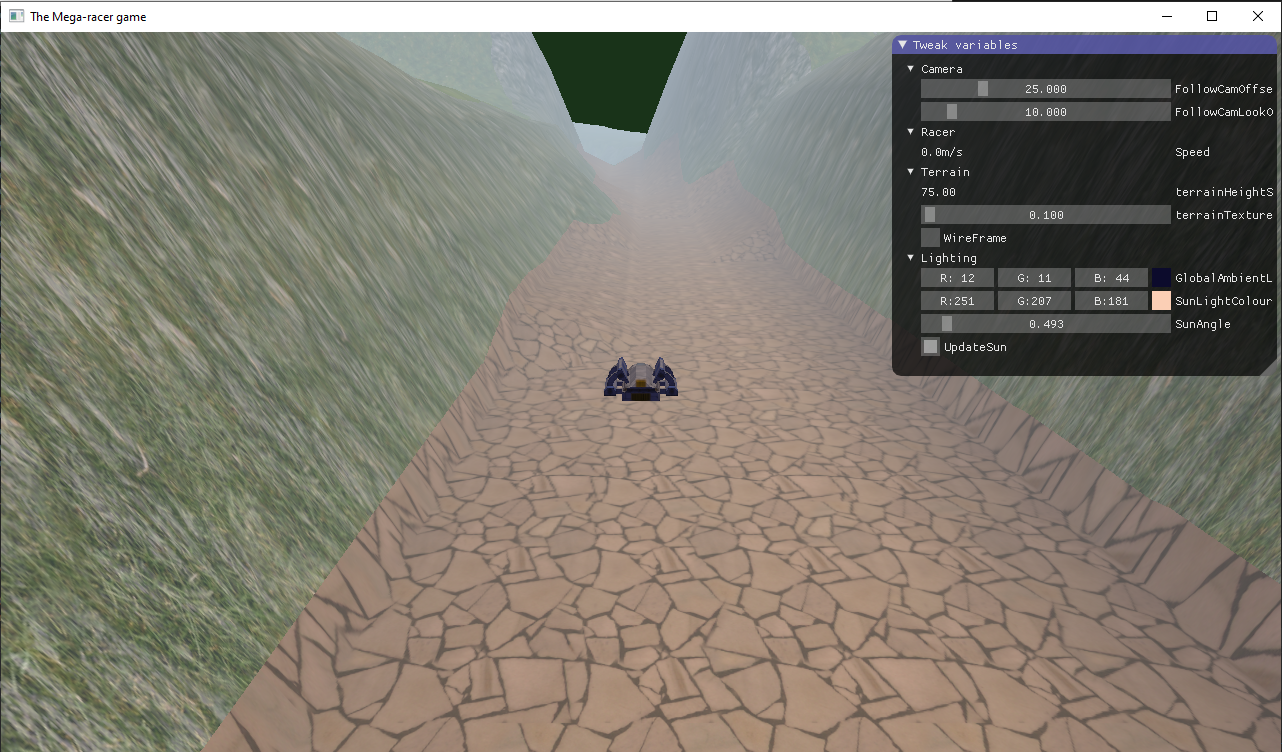
\includegraphics[width=0.49\textwidth, frame]
        {./images/mega_racer/2.2_a_1.PNG}%
    \hfill
    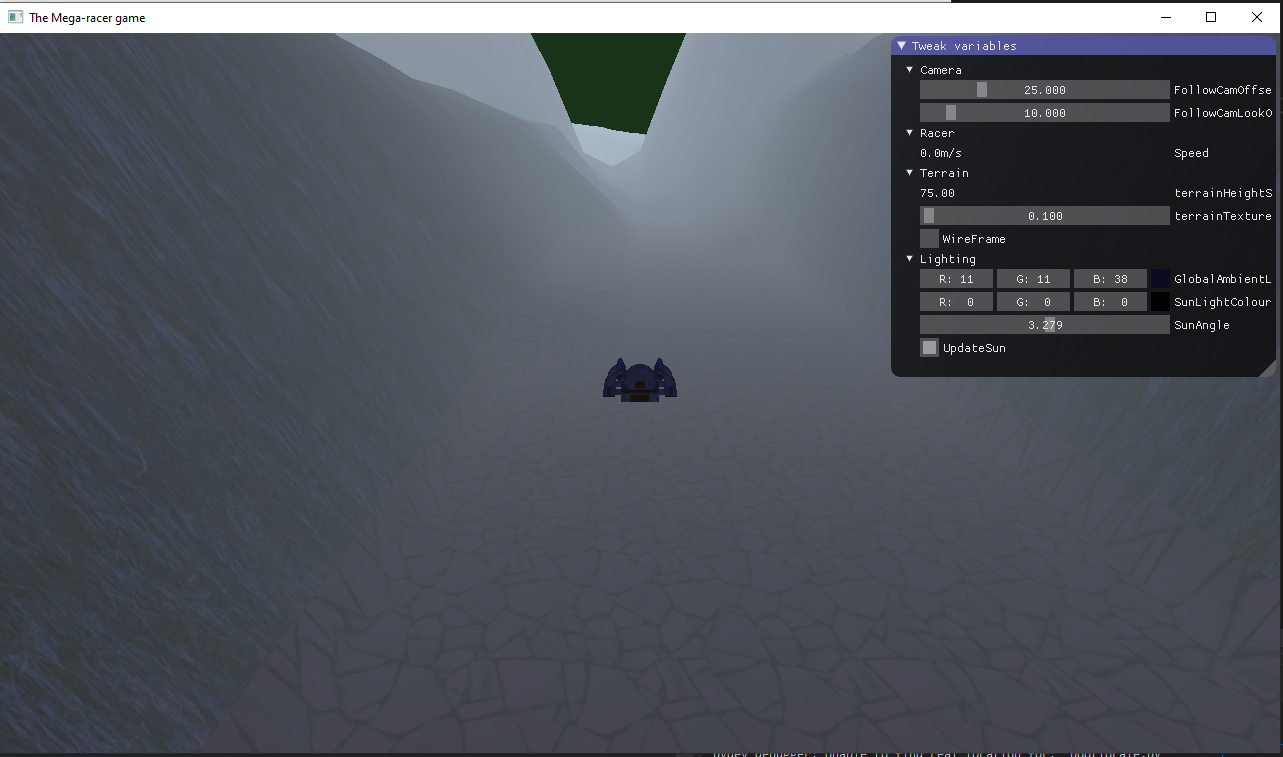
\includegraphics[width=0.49\textwidth, frame]
        {./images/mega_racer/2.2_a_2.PNG}        
    }        
    \caption{2.2 - Basic}   
\end{figure}


\textbf{(2) Make colour sunLight and Ambient}: As evident in the screenshots, this implementation of fogColour is not correct, especially when there is no direct sunlight. Following the advice of the project notes, a combination of the sunLightColour and ambientColour were trialled. 

First, the these two values were added together.
\begin{lstlisting}
    vec3  fogColor  = (sunLightColour + globalAmbientLight)
\end{lstlisting} 

\begin{figure} [H]
    \makebox[\textwidth]{%
    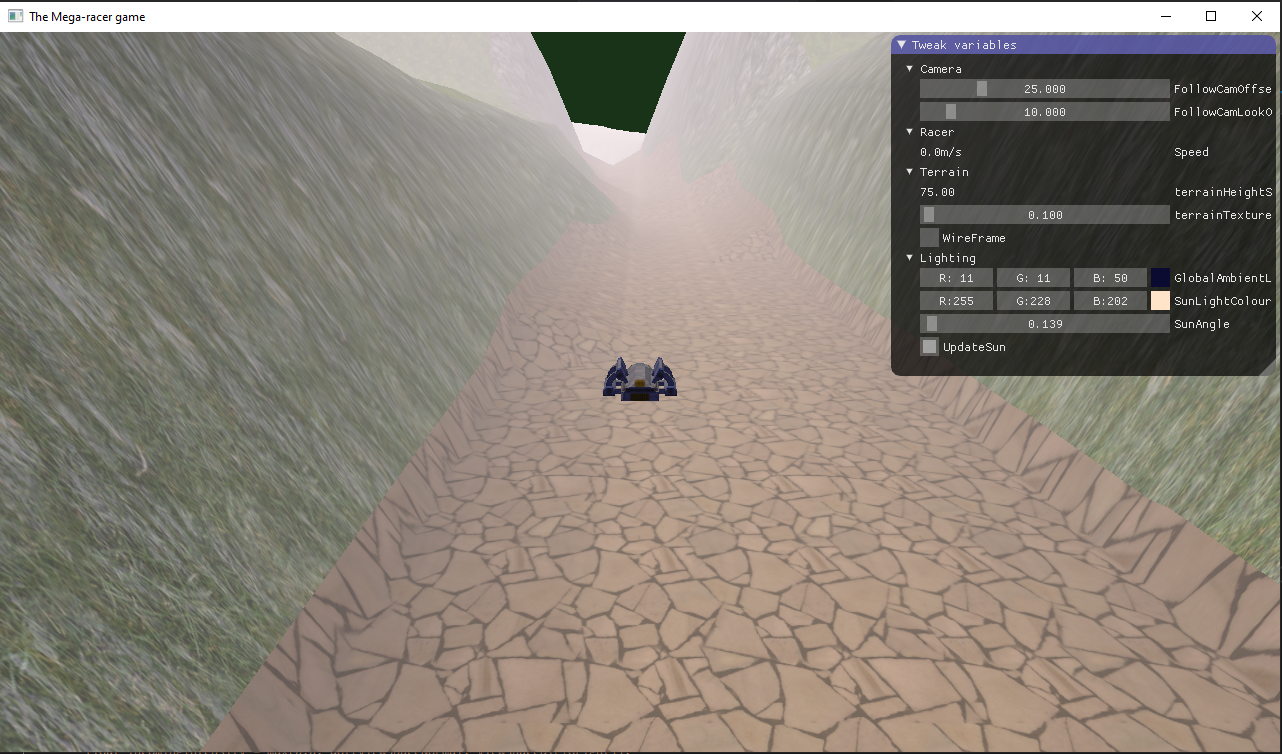
\includegraphics[width=0.49\textwidth, frame]
        {./images/mega_racer/2.2_b_1.PNG}%
    \hfill
    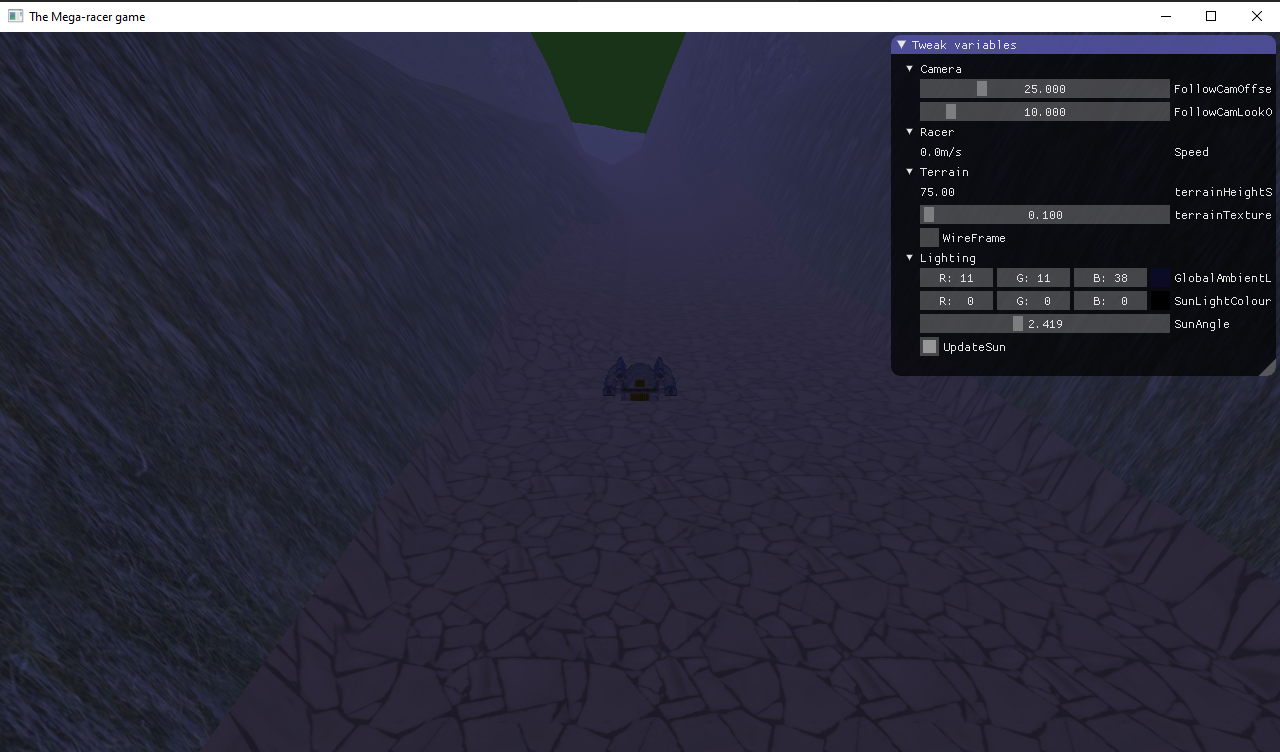
\includegraphics[width=0.49\textwidth, frame]
        {./images/mega_racer/2.2_b_2.PNG}        
    }        
    \caption{2.2 - Fog Colour (Total)}   
\end{figure}

Then an average of the two values was tested, which produced a less grey result and was the best combination at this stage.
\begin{lstlisting}
    vec3  fogColor  = (sunLightColour + globalAmbientLight) / 2.0
\end{lstlisting}

\begin{figure} [H]
    \makebox[\textwidth]{%
    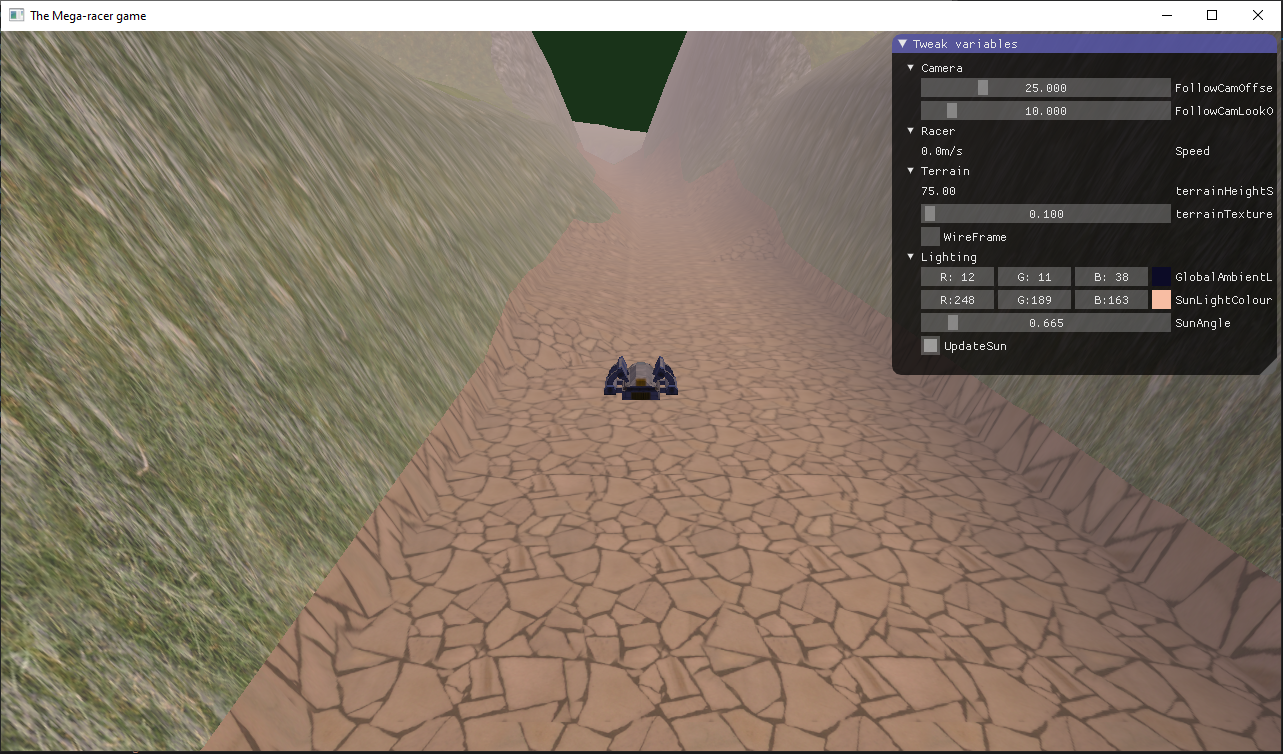
\includegraphics[width=0.49\textwidth, frame]
        {./images/mega_racer/2.2_c_1.PNG}%
    \hfill
    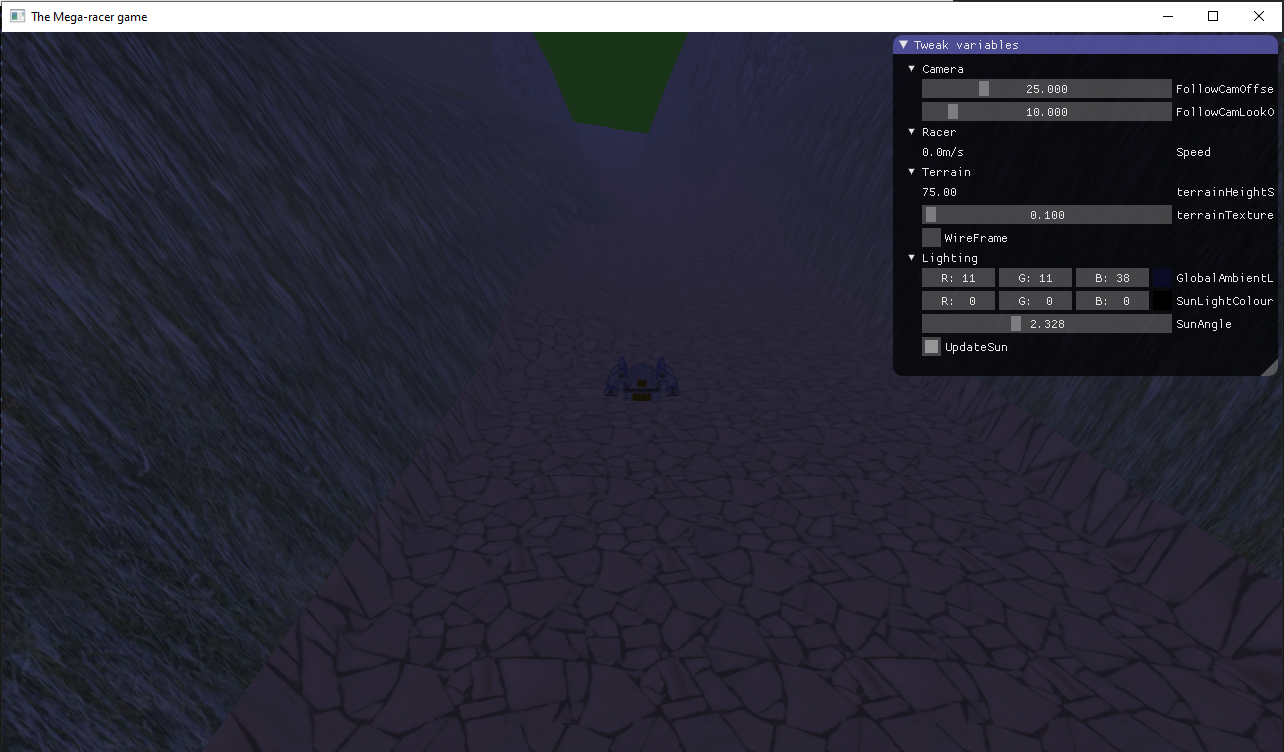
\includegraphics[width=0.49\textwidth, frame]
        {./images/mega_racer/2.2_c_2.PNG}        
    }        
    \caption{2.2 - Fog Colour (Average)}   
\end{figure}

\textbf{(3) Height based}
To take the fog one step further, the height based fog implementation from the provided tutorial was implemented. Now as well as creating a fog appearance that doesn't have a constant colour, the fog will also not have a constant density. This essentially means the intensity of the fog colour changes with distance and height to create a more interactive fog appearance so areas further away have more fog intensity. The \textit{applyFog()} function will be updated with this implementation and same as before, the call to the function also needs to be updated in fragmentShader. There are a few more variables needed as well:
    \begin{itemize}
        \item cameraPosition = The position of the camera in the world space, using the coordinates of \textit{worldToViewTransform} 
        \item cameraToPointVector = normalize(positionIn - cameraPosition);
    \end{itemize}

    \begin{lstlisting}
# Tutorial
vec3 applyFog( in vec3  rgb,      // original color of the pixel
                in float distance, // camera to point distance
                in vec3  rayOri,   // camera position
                in vec3  rayDir )  // camera to point vector
{
    float fogAmount = c * exp(-rayOri.y*b) 
                        * (1.0-exp( -distance*rayDir.y*b ))/rayDir.y;
    vec3  fogColor  = vec3(0.5,0.6,0.7);
    return mix( rgb, fogColor, fogAmount );
}
-->
# mega_racer.py - Rendering system
commonFragmentShaderCode = 
    ...
    vec3 applyFog(in vec3 rgb, in float distance, in vec3  rayOri, in vec3 rayDir)
    {
        float b = 0.005;
        float c = 0.66;
        float fogAmount = c * exp(-rayOri.y*b) 
                            * (1.0-exp( -distance*rayDir.y*b ))/rayDir.y;
        vec3  fogColor  = (sunLightColour + globalAmbientLight) / 2.0;
        return mix( rgb, fogColor, fogAmount );
    }

# terrain.python
def load(...):
    ...
    vertexShader =
        ...
        uniform mat4 worldToViewTransform;

        out VertexData
        {
            ...
            vec3 cameraPosition;
            vec3 cameraToPointVector;
        }
        void main()
        {
            ...
            cameraPosition = vec3(worldToViewTransform[3][0],
                                    worldToViewTransform[3][1],
                                    worldToViewTransform[3][2])
            cameraToPointVector = normalize(positionIn - cameraPosition);
            ...
        }
    fragmentShader = 
        in VertexData
        {
            ...
            vec3 cameraPosition;
            vec3 cameraToPointVector;
        }
        void main()
        {
            ...
            fragmentColor = vec4(toSrgb(applyFog(reflectedLight, 
                                            -v2f_viewSpacePosition.z, 
                                            cameraPosition, 
                                            cameraToPointVector)), 1.0);
        }
    \end{lstlisting} 
\begin{figure} [H]
    \makebox[\textwidth]{%
    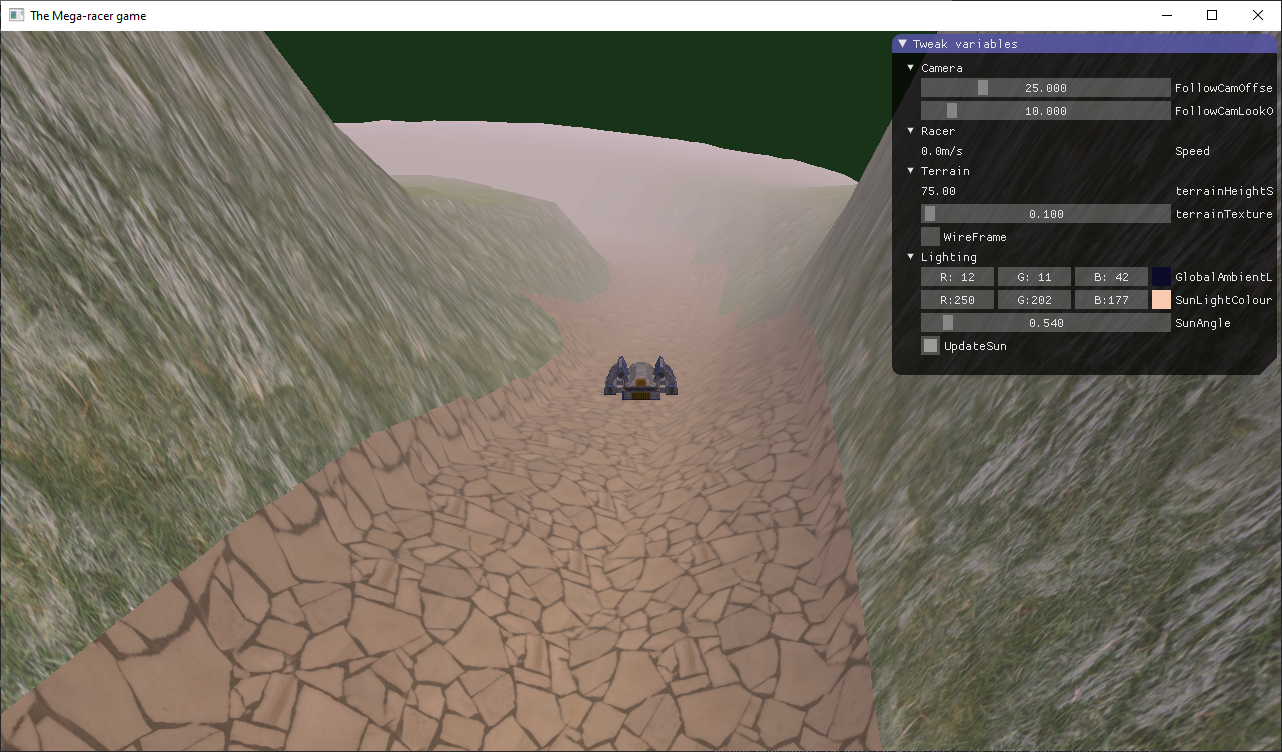
\includegraphics[width=0.49\textwidth, frame]
        {./images/mega_racer/2.2_d_1.PNG}%
    \hfill
    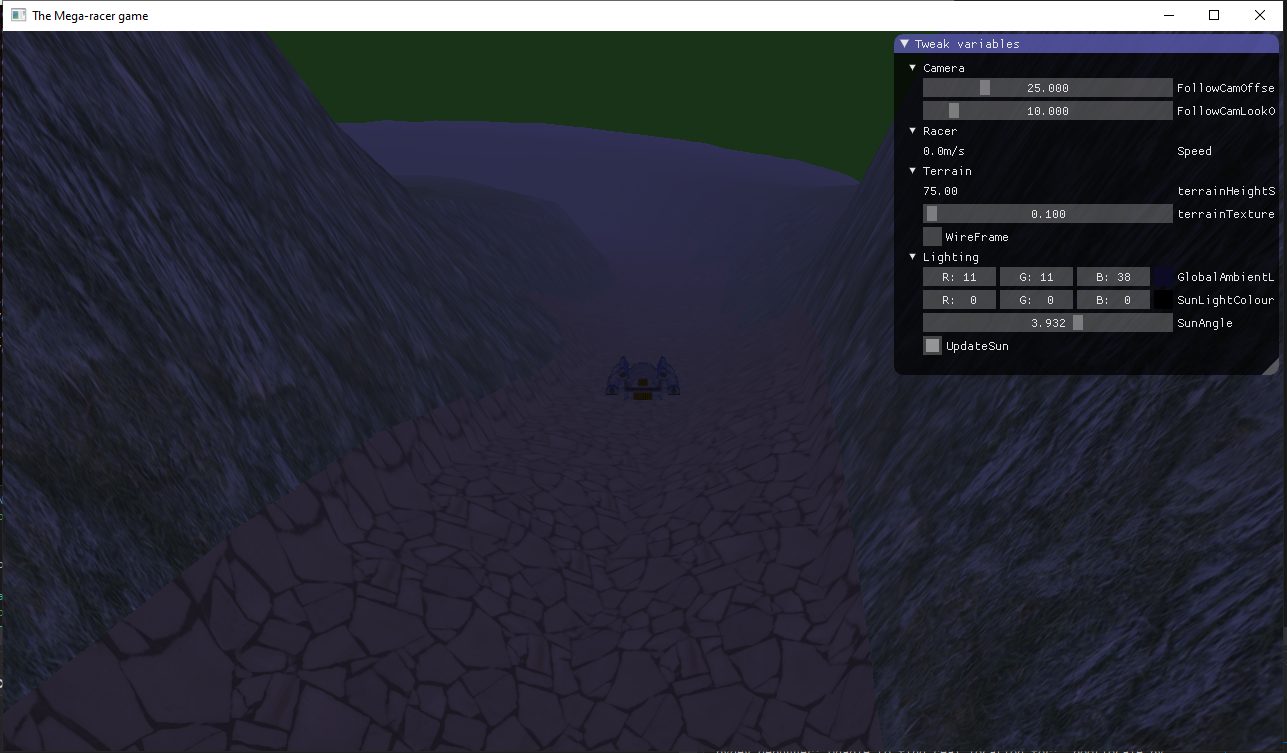
\includegraphics[width=0.49\textwidth, frame]
        {./images/mega_racer/2.2_d_2.PNG}        
    }        
    \caption{2.2 - Height Fog}   
\end{figure}


% 2.3
\subsubsection{2.3 Props}
Introducing other objects into the world, such as trees and rocks, creates a more realistic and fun environment. The logic related to generating the locations of trees and rocks have already been handed in terrain.py by load(). This is dependent on the value of the green pixel, the coordinate from the map is saved to the relevant prop list. Several object model files have also been provided in the data folder.

\textbf{(1) Create the Prop class}
A new prop.py file was created and a Prop class declared. The props are an object just like the racer, so to get a foundation, the Racer class from racer.py was referenced heavily. To start with all of the same libraries were imported and all of the variables copied over. From here any variables that were not required were removed (velocity, speed, maxSpeedRoad, maxSpeedRough, terrain) and new variables added (rotation). Next the render() and load() functions from the Racer class were copied (update() is not required since once created the elements of the props don't change).
    \begin{lstlisting}
# prop.py
import libraries....

class Prop:
    position = vec3(0,0,0)    
    heading = vec3(1,0,0)
    rotation = 0.0

    zOffset = 3.0
    angvel = 2.0
    
    model = None
    \end{lstlisting}

The load() function stills needs to assign the variables of each prop instance as it did in the racer, however a few things of changed. First of all the terrain variable is no longer needed. Secondly, the position is randomised from a given list based on the prop type, as well as the rotation. This is achieved by importing the 'random' library and using choice() which randomly selects an entry from a list [49]. Finally, the model of each unique prop should only be loaded once. The model for each prop type will be created in a prop manager class and then passed in to each instance of that prop type.
    \begin{lstlisting}
#prop.py - Prop
import random

def load(self, model, locations):      
    self.position = random.choice(locations)
    self.rotation =random.choice(range(0,360))
    self.model = model
    \end{lstlisting}

The render() function needed to follow the same steps from Racer.render(), as well as apply the random rotation of props in the world. The only difference is that when calling drawObjModel() the modelToWorldTransform parameter is multiplied by a matrix construction function (defined in lab\_utils.py) based on the random rotation as the angle argument. 
    \begin{lstlisting}
#prop.py - Prop
def render(self, view, renderingSystem):
    modelToWorldTransform = lu.make_mat4_from_zAxis(self.position,
                                                     self.heading, 
                                                     [ 0.0, 0.0, 1.0 ])
    rotationMatrix = lu.make_rotation_y(self.rotation)
    renderingSystem.drawObjModel(self.model, 
                                    modelToWorldTransform * rotationMatrix, 
                                    view)
    \end{lstlisting}
 
\textbf{(2) Create the PropManager class}
Now, that the Prop class has been created the next step was to create a class to manage all of the prop instances; PropManager. To start the required variables were declared. For each prop type there needed to be a maximum number of instances, a list to keep track of the instances, a single model.
    \begin{lstlisting}
# prop.py
class PropManager: 
    treeMax = 50
    treeList = []
    treeModel = None

    rockMax = 20
    rockList = []
    rockModel = None
    \end{lstlisting} 

Now to create the instances of each prop type and save them in a global list (treeList or rockList). The process is the same for all prop types so a general function, loadPropList(), creates the instances for the prop type and fills the list. For each prop type, there are max number of instances (propMax). Each of these instances uses a single model of the prop type (propModel) with a position from the designated list for that prop type (propLocations). The instance is then appended to the relevant list for easier access (propList). 
    \begin{lstlisting}
# prop.py - PropManager
def loadPropList(self, propModel, propMax, propLocations):
propList = []
i = 0
while i < propMax:
    prop = Prop()
    prop.load(propModel, propLocations)
    propList.append(prop)            
    i += 1
    print(prop.position)
return propList
    \end{lstlisting} 

This function is called for each prop type, with their specific values, and assigned to the relevant prop type list in loadAllProps(), after first creating the unique model for each prop type in loadAllProps(). This means the model for each prop is created only once and all instances share the same model (i.e. textures, vector data, etc). 
    \begin{lstlisting}
# prop.py - PropManager 
def loadAllProps(self, terrain): 
    # Load trees
    self.treeModel = ObjModel("data/trees/birch_01_d.obj")
    self.treeList = self.loadPropList(self.treeModel, self.treeMax, 
                                        terrain.treeLocations)
    # Load rocks
    self.rockModel = ObjModel("data/rocks/rock_01.obj")
    self.rockList = self.loadPropList(self.rockModel, self.rockMax, 
                                        terrain.rockLocations)
    \end{lstlisting}

As well as loading the props, the props will need to have a function call that renders them as well in the same way as other object models in that each prop instance is rendered individually using render().
\begin{lstlisting}
# prop.py - PropManager 
def renderAllProps(self, view, renderingSystem):
    for prop in self.allProps:
        prop.render(view, renderingSystem)
\end{lstlisting}

\textbf{(3) Place in the world}
With the PropManager defined the props can now be loaded in the world. The PropManager class needs to be imported and the variable created. Then, below were the g\_racer and g\_terrain are being assigned as instances of their corresponding class' and loaded, the same needs to be done for the props as g\_props.Additionally, all of the props also needed to be rendered, again in the same area as the g\_racer and g\_terrain variables are rendered.
    \begin{lstlisting}
#mega_racer.py
from prop import PropManager
...
g_props = None
....
g_props = PropManager()
g_props.loadAllProps(g_terrain)
...
def renderFrame(...):
        ...
        g_props.renderAllProps(view, g_renderingSystem)
    \end{lstlisting}

    \begin{figure} [H]
        \centering
        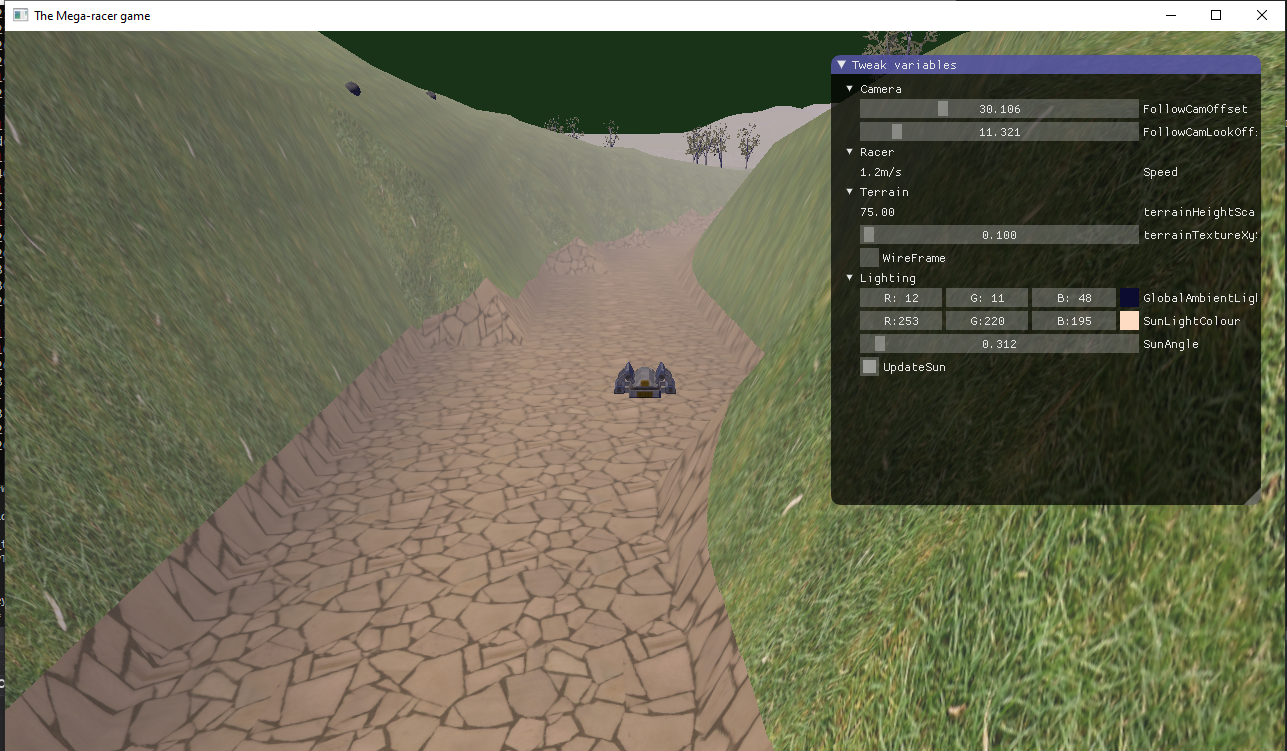
\includegraphics[width=0.8\textwidth, frame]
            {./images/mega_racer/2.3.PNG}  
        \caption{2.3 - Props (trees and rocks)}   
    \end{figure}


%%%%% OLYMPIC STADIUM %%%%%
\section{Olympic Stadium}
The most important area at an Olympics is the main Olympic Stadium where the athletic track is located. With the foundation of the mega racer implemented, this section was an opportunity to test my knowledge in a new environment, learn about graphic modelling software and try some advanced computer graphic techniques.

\textbf{Modifications:} The following are the changes, in order, that were made to the Mega Racer game in order to create an Olympic Stadium.
\begin{enumerate}
    \item Car Model: Race Car  $\dashrightarrow$ Athlete running    
    \item Props: Trees, Rocks $\dashrightarrow$ Cones, Rings, Podium
    \item Terrain Textures: Grass, Paving, Rock Steep, Rock High $\dashrightarrow$ Grass, Synthetic track, Concrete, Seats
    \item Track: Racing track in wilderness $\dashrightarrow$ Olympic Stadium with athletic track
\end{enumerate}

\textbf{Setup:} To get started these steps were first taken:
\begin{enumerate}
    \item Create a duplicate copy of mega\_racer.py
    \item Rename mega\_racer.py to olympic\_stadium.py
    \item Change the window title to "The Olympic Stadium Tour"

    \begin{lstlisting}
window = glfw.create_window(g_startWidth, g_startHeight, 
                                "The Olympic Stadium Tour", None, None)
\end{lstlisting}
\end{enumerate}

\textbf{Blender:} In the process of changing elements in the mega\_racer world to reflect an Olympic stadium all of the object models (.obj and .mtl) needed to be either created or modified in blender. This was either because an appropriate free .obj file could not be found or was scaled incorrectly, and/or the .mtl file was missing or not correct. Some basics that needed to be learned to get started was scaling [1] and rotating [2] tutorials.

\subsection{Athlete}
Instead of a race car driving around the track, I wanted to replace it with an athlete. A person is quite a complicated model to make from scratch so a premade .obj model of a basic person was sourced. The chosen model was [35], a free basic mesh male model uploaded by Paul Chen. The model is in a basic standing position with no texturing. For a more realistic model for the stadium, the model needed to be scaled appropriately and posed in a running position. Importing the .obj file in blender and following a basic rigging tutorial on YouTube by PIXXO 3D [10], a meta-rig was set up for the model. This basically entails lining up a bone framework, like a skeleton, to the model. One of the errors that occurred was was moving one of the spine bones on accident so that it was detached disallowing the meta-rig from generating, however it was solved by reattaching the bones [40].
    \begin{figure} [H]
        \makebox[\textwidth]{%
        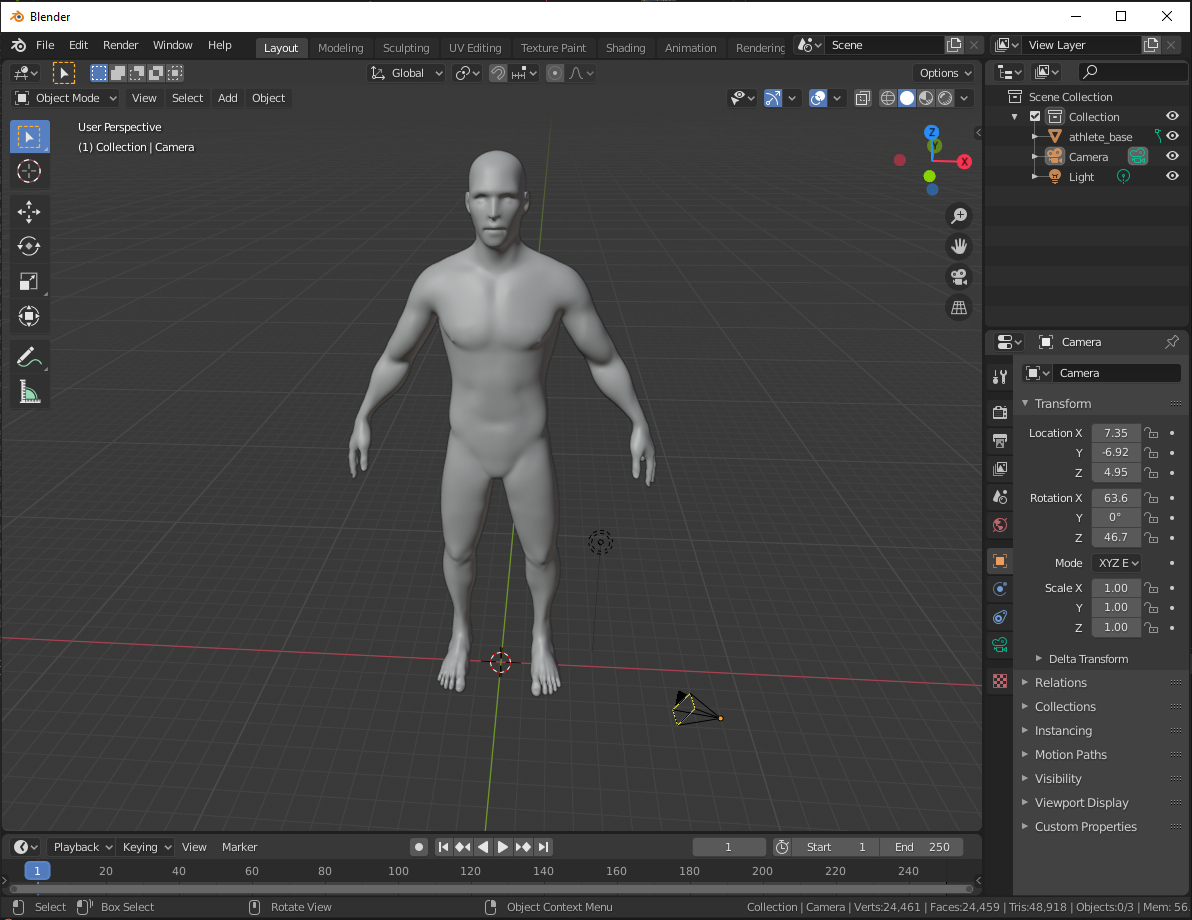
\includegraphics[width=0.49\textwidth, frame]
            {./images/olympics/athlete_blend_base.PNG}%
        \hfill
        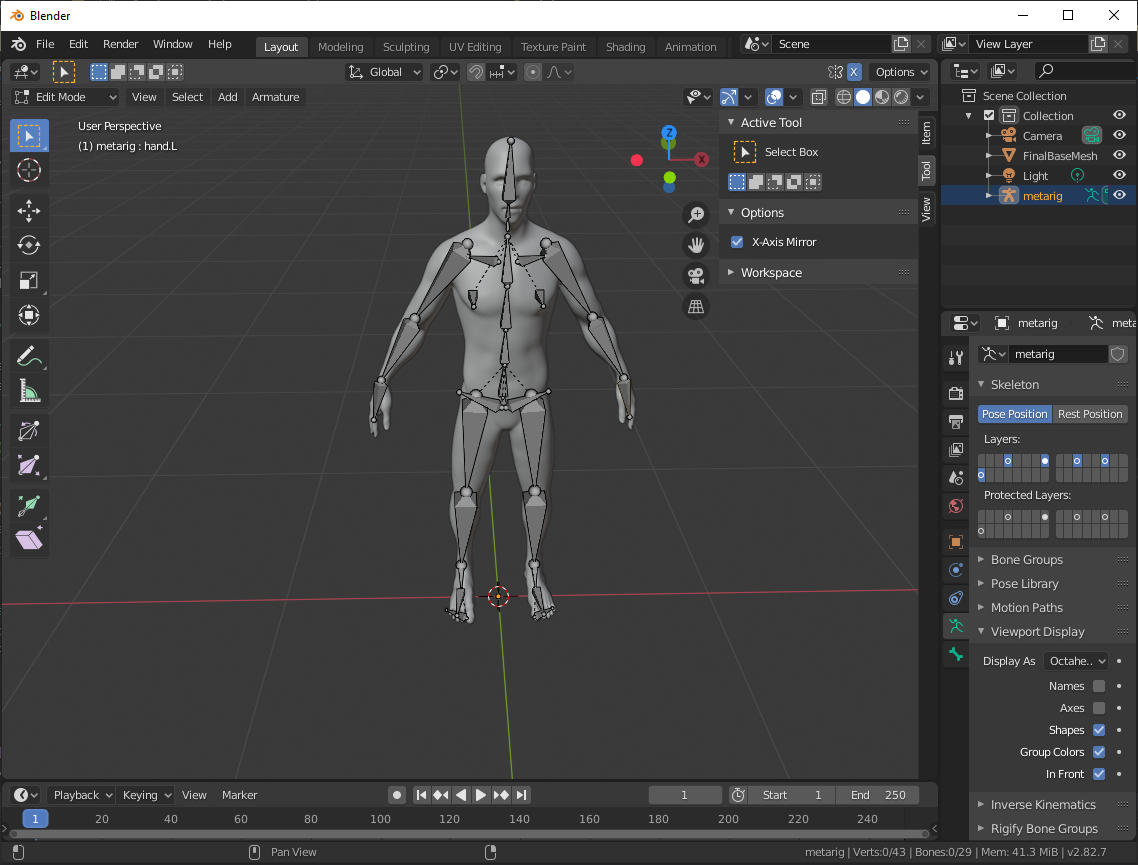
\includegraphics[width=0.49\textwidth, frame]
            {./images/olympics/athlete_blend_metarig.PNG}        
        }        
        \caption{Racer - Blender - Base \& Rig}   
    \end{figure}

Using this meta-rig, blender has a built-in feature that creates a rig that can be used to move the 'bones' around to place the model into poses. For the model, one leg needed to be lifted backward from the knee and point the foot down, and slightly lift the other foot and bend the knee slightly forward. The arms were moved in the same fashion with one arm back and the hand pointing down and the other arm forward with bend elbow and hand pointing up. Essentially, this put the model in a running pose.
    \begin{figure} [H]
        \makebox[\textwidth]{
        \centering
        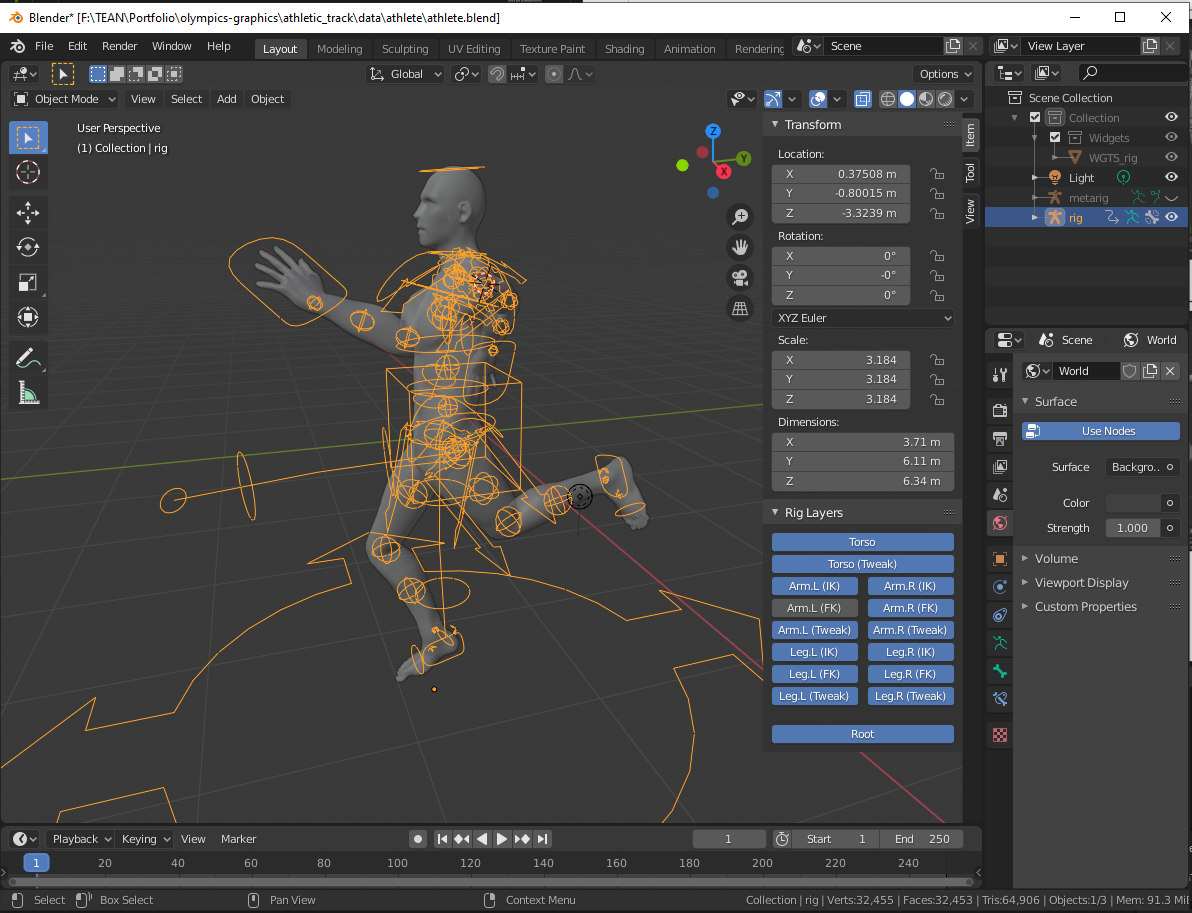
\includegraphics[width=0.49\textwidth, frame]
            {./images/olympics/athlete_blend_rig2.PNG}
        \hfill
        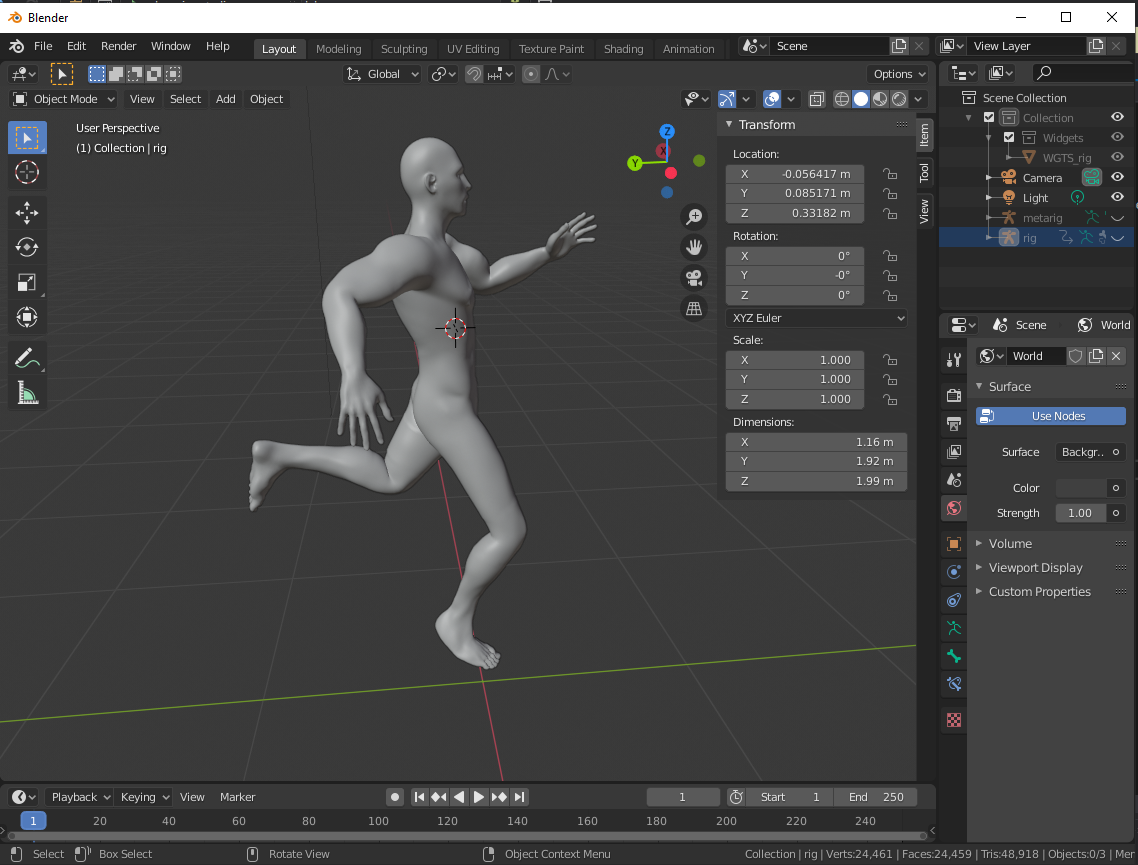
\includegraphics[width=0.49\textwidth, frame]
            {./images/olympics/athlete_blend_pose.PNG}        
        }        
        \caption{Racer - Blender - Posing}   
    \end{figure}

Now that the athlete was in the running position, some texturing needed to be added. Sourcing images from Google, some textures were found that were appropriate for an athlete including Lycra and breathable material. However, since the model was set as all one material, vertex groups would be needed to be used in order to separate them into different sections by following a tutorial from Jayanam [7]. In this step, I would have liked to have learn to extrapolate the areas to give them definition and shape the areas to look as they should i.e. make the feet look like shoes. For this basic model, after creating the groups  they were able to be coloured separately by assigning the different materials (sourced image textures) to the groups as done by Weisbrod Imaging [14].
    \begin{figure} [H]
        \makebox[\textwidth]{%
        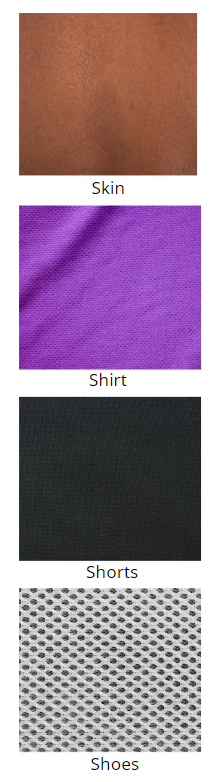
\includegraphics[width=0.15\textwidth, height=0.41\textheight, frame]
            {./images/olympics/athlete_textures.PNG}%
        \hfill
        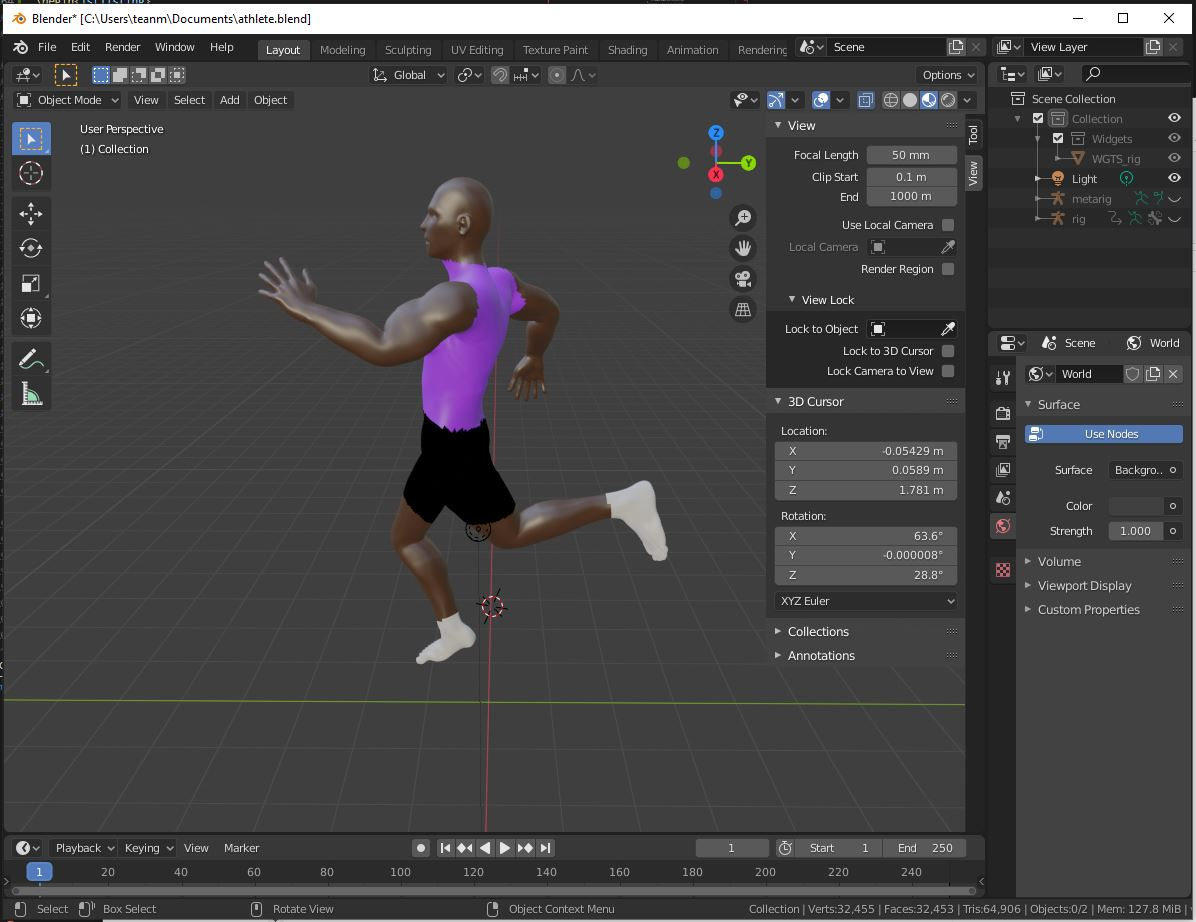
\includegraphics[width=0.8\textwidth, frame]
            {./images/olympics/athlete_blend_colour.jpg}        
        }        
        \caption{Racer - Blender - Colour}   
    \end{figure}

The athlete was coming together. However, I really didn't like the dodgy colouring attempt so I decided to try and add clothing for more realistic texturing. The following free clothing models were found on turbosquid.com:
\begin{itemize}
    \item \textbf{Men Avatar Vest} by swatishr13 [28]: This model was imported with no colouring associated. The trims on the sleeve were set as white and the main colour used the same 'top' texture as in the previous colouring. 
    \item \textbf{short pants} by sazandra [29]: This file was able to be imported with all textures correctly. Since the model was in a running position, the pants were the wrong shape however the model used a mirror modify so the model was able to be split and just have half of the pants. This half of the pants were used as is and then duplicate was made with a mirror image of the local x and y coordinates that could be set at the right shape for the runner.
    \item \textbf{shoe} by Bruno Dalla [22]: This model is of a single show so a duplicate mirrored on the local x was created. The associated texturing for this model didn't load correctly so the above 'shoe' texturing was used except for a trim around the bottom the same colour as the top.
\end{itemize}


\begin{figure} [H]
    \centering
    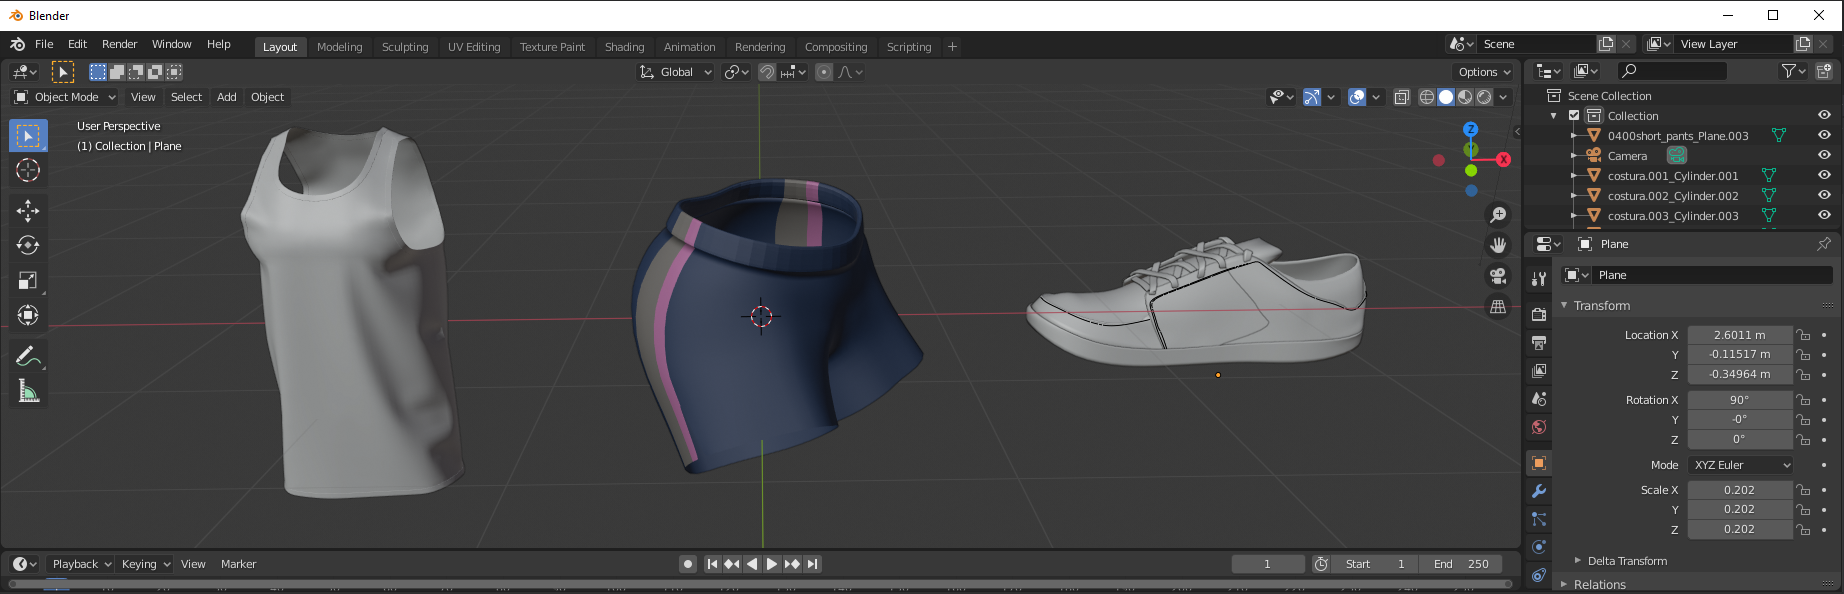
\includegraphics[width=0.9\textwidth, frame]
        {./images/olympics/athlete_clothes_base.PNG}
    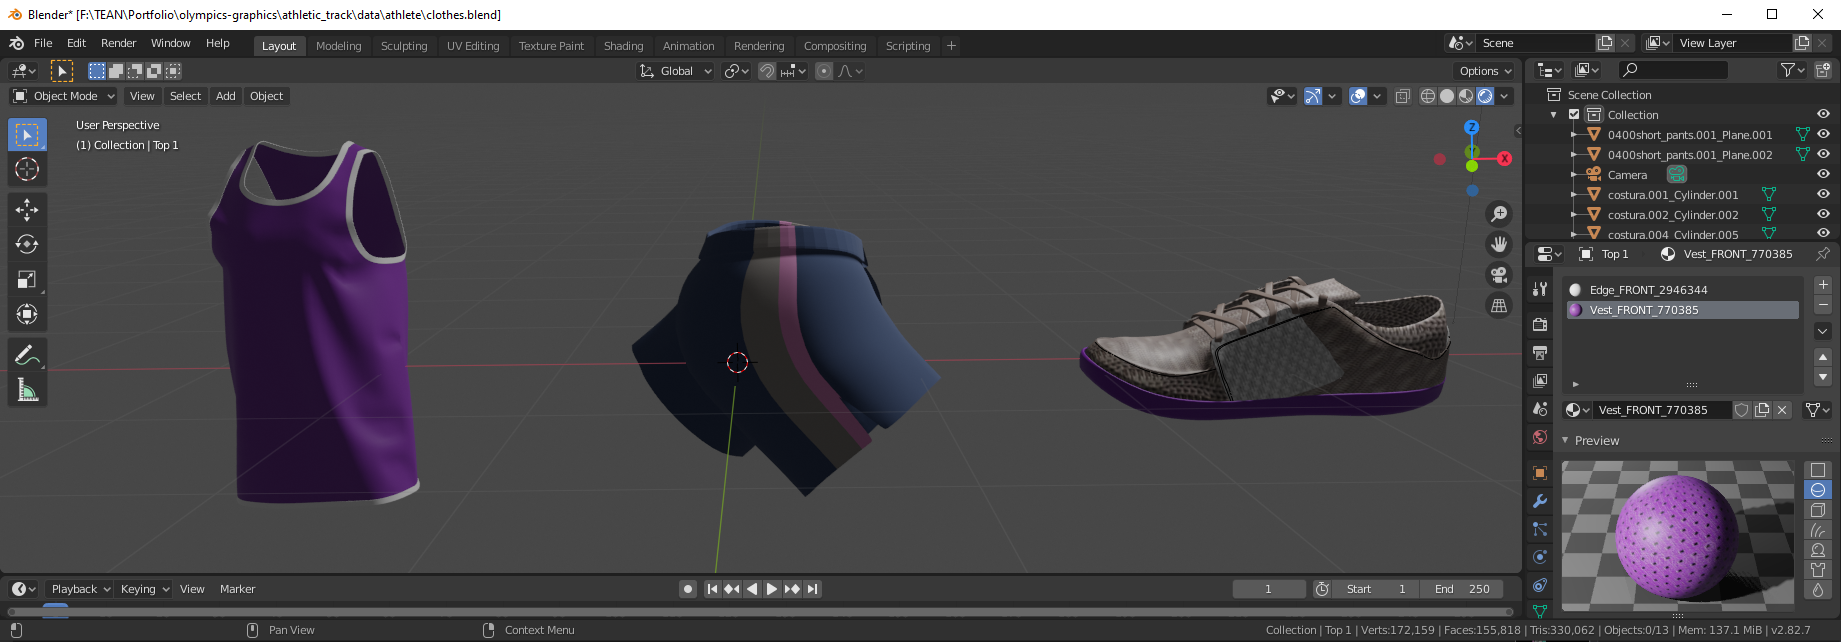
\includegraphics[width=0.9\textwidth, frame]
        {./images/olympics/athlete_clothes_colour.PNG}    
    \caption{Racer - Blender - Clothes}   
\end{figure}

The human model is now complete with clothes and posed. The next step would be to add skin texturing and more human features. This was a level of detail that was beyond my ability for this project. Perhaps another time.
\begin{figure} [H]
    \centering
    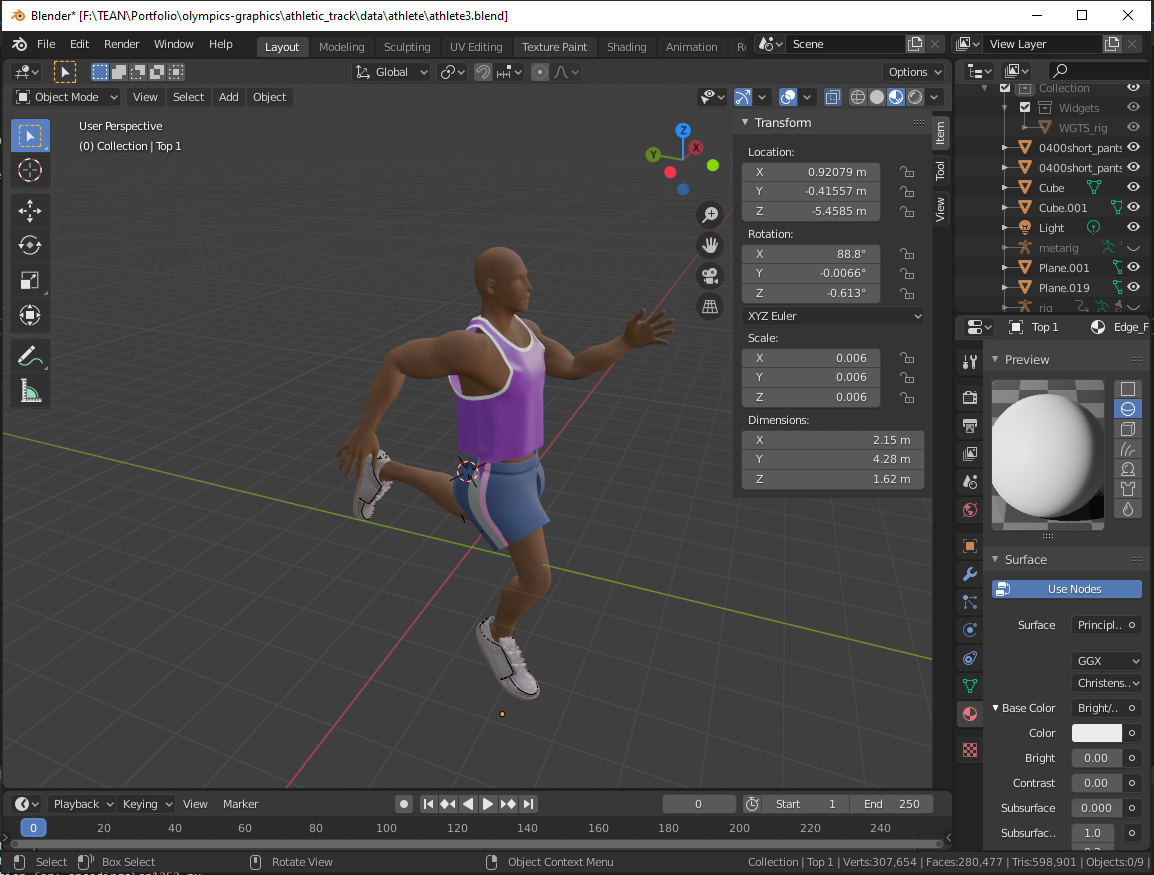
\includegraphics[width=0.8\textwidth, frame]
        {./images/olympics/athlete_blend_clothes.PNG}  
    \caption{Racer - Blender - Final}   
\end{figure}

Finally, the athlete was placed in the world to scale. The name of the athlete was kept as g\_racer/racer throughout code as this is appropriate for the context but instead of the racer\_01.model the new athlete.obj file imported.
\begin{lstlisting}
#mega_racer.py    
g_racer.load("data/athlete/athlete.obj", g_terrain, g_renderingSystem);
\end{lstlisting}

\begin{figure} [H]
    \centering
    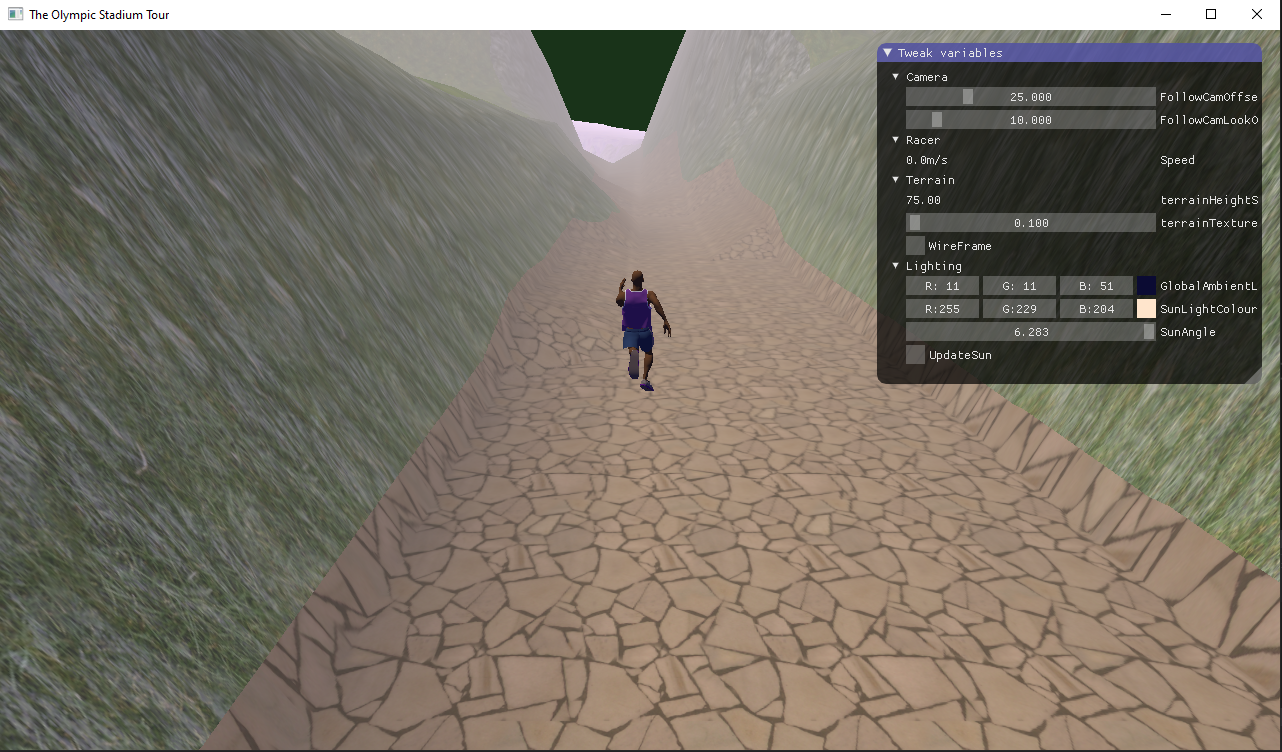
\includegraphics[width=0.8\textwidth, frame]
        {./images/olympics/athlete_world.PNG}  
    \caption{Athlete}   
\end{figure}


\subsection{Props}
Since an Olympic Stadium is essentially a building, trees and rocks were note appropriate models to keep in the world. With some blender experience now obtained, the props for this implementation were made from scratch with the assistance of tutorials. Originally, these models were going to be sourced from online libraries such as turbosquid.com, free3d.com, cgtrader.com and opengameart.org, however after searching the models were not complete, inadequate or difficult to find. Making these models was an interesting experience as it gave me the experience of the quality and detail of texturing, shaping, scaling, shading and lighting of 3D graphic models. As well as as better understanding of how the .obj files were handled, manipulated and created, along with their accompanying .mtl file. The props that were created were Olympic Rings (to replace rocks) and safety cones (to replace trees). 

Additionally, the code for this section was updated as originally more models were planned to be included. This code is very similar to mega racer though handles more types of props. Other props that were considered were a podium, hurdles, Olympic flame and crowd members.

\begin{lstlisting}
#mega_racer.py
propTypes = [['cone', 50, g_terrain.treeLocations], 
            ["rings", 2, g_terrain.rockLocations]]
g_props.loadAllProps(propTypes)

#prop.py
class PropManager: 
    propTypes = []
    allProps = []    

    def loadProp(self, propType):
        propModel = ObjModel("data/{propName}/{propName}.obj"
                        .format(propName=propType[0]))
        i = 0
        while i < propType[1]:
            prop = Prop()
            prop.load(propModel, propType[2])         
            i += 1
            self.allProps.append(prop)

    def loadAllProps(self, propTypes):
        self.propTypes = propTypes
        for prop in self.propTypes:
            self.loadProp(prop)

    def renderAllProps(self, view, renderingSystem):
        for prop in self.allProps:
            prop.render(view, renderingSystem)    
    \end{lstlisting}

    \begin{figure} [H]
        \centering
        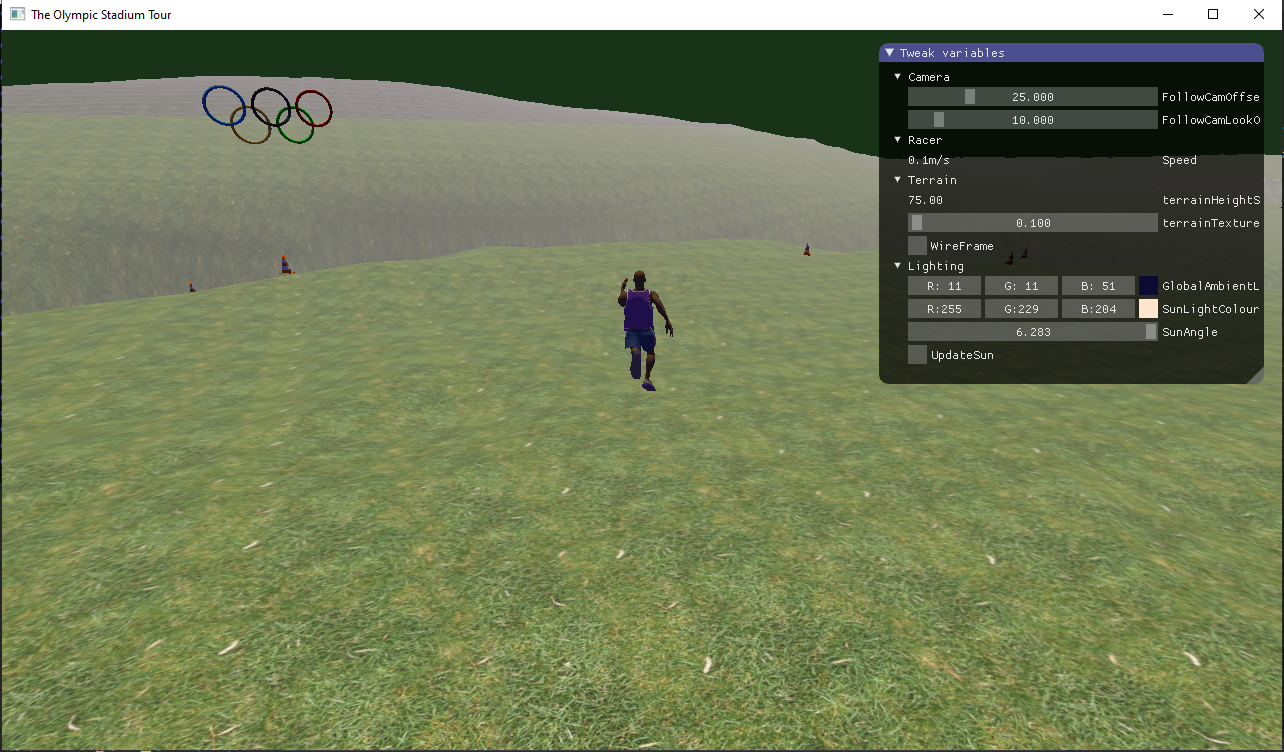
\includegraphics[width=0.8\textwidth, frame]
            {./images/olympics/props_world.PNG}  
        \caption{Athlete}   
    \end{figure}
        
\subsubsection{Rings}
It wouldn't be the Olympics without the iconic Olympic rings. Originally a free model was sourced [21], however after trying to open it in blender not only were the set materials not working from the .mtl file but also the rings were connected and overlapping so I wasn't able to separate them out to colour them differently. They seemed simple enough to make myself so following a time-lapse video [4]and sourcing my own textures for the rings to make a new model that could be used on the centre area of the stadium. Each ring is a torus that was reshaped slightly, coloured with the textures and then overlapped with the two bottom rings in front. 
    \begin{figure} [H]
        \makebox[\textwidth]{%
        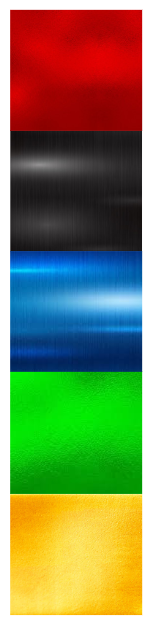
\includegraphics[width=0.15\textwidth, height=0.41\textheight, frame]
            {./images/olympics/rings_textures.PNG}%
        \hfill
        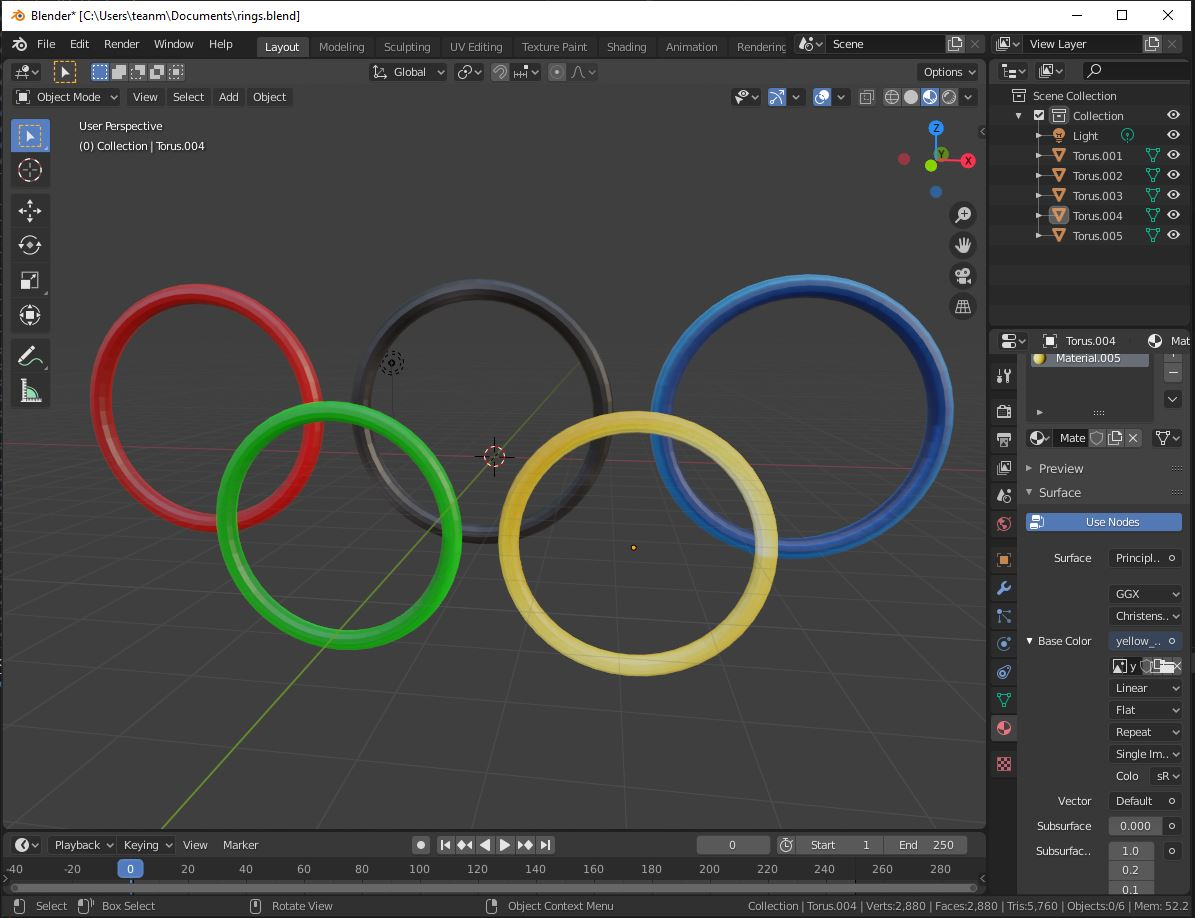
\includegraphics[width=0.8\textwidth, frame]
            {./images/olympics/rings_blend.jpg}        
        }        
        \caption{Props - Rings}   
    \end{figure}

\subsubsection{Cones}
To demonstrate props that would be repeated on a large scale, safety cones were placed around the inside of the middle area of the stadium. Similar to the Olympic rings, various models [30] were found but the .mtl file was not correct for any of them, so I decided to create my own cones. Following a tutorial [8], a realistic traffic safety cone was created. The cone started as a cylinder, the top was reshaped for the cone appearance, the lip on the top was created, a base added, the strips added using loop cuts and finally the colouring applied.
    \begin{figure} [H]
        \centering
        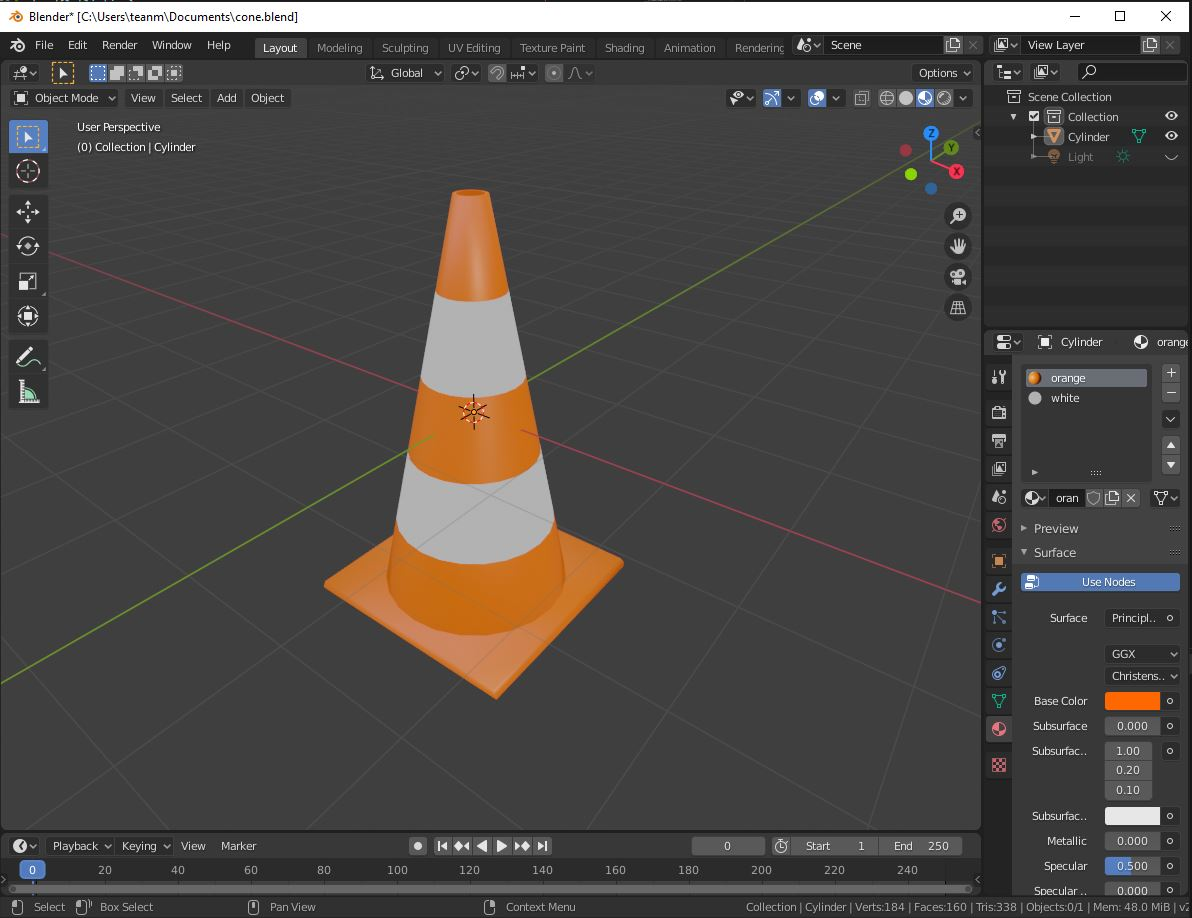
\includegraphics[width=0.8\textwidth, frame]
            {./images/olympics/cone_blend.jpg}
        \caption{Props - Cone}   
    \end{figure}

% MAP
\subsection{Map}
The current map does not resemble a stadium at all so I wanted to attempt to create my own map using Paint. The track needed to be to scale by using dimensions of an athletic track [23] and stadium [31]. After trialling with a few image pixel sizes, I decided to optimise the RGB image quality by multiplying all measurements (in metres) by 2 pixels. Since Paint is very low quality using the original 128x128 caused too much interference with the 'smoothness' of the 'stadium' shape of the track, 1 to 1 scaling proved problematic with object models scaling and anything larger was too difficult to render. This was the happiest medium.
 
\begin{figure} [H]
    \centering
    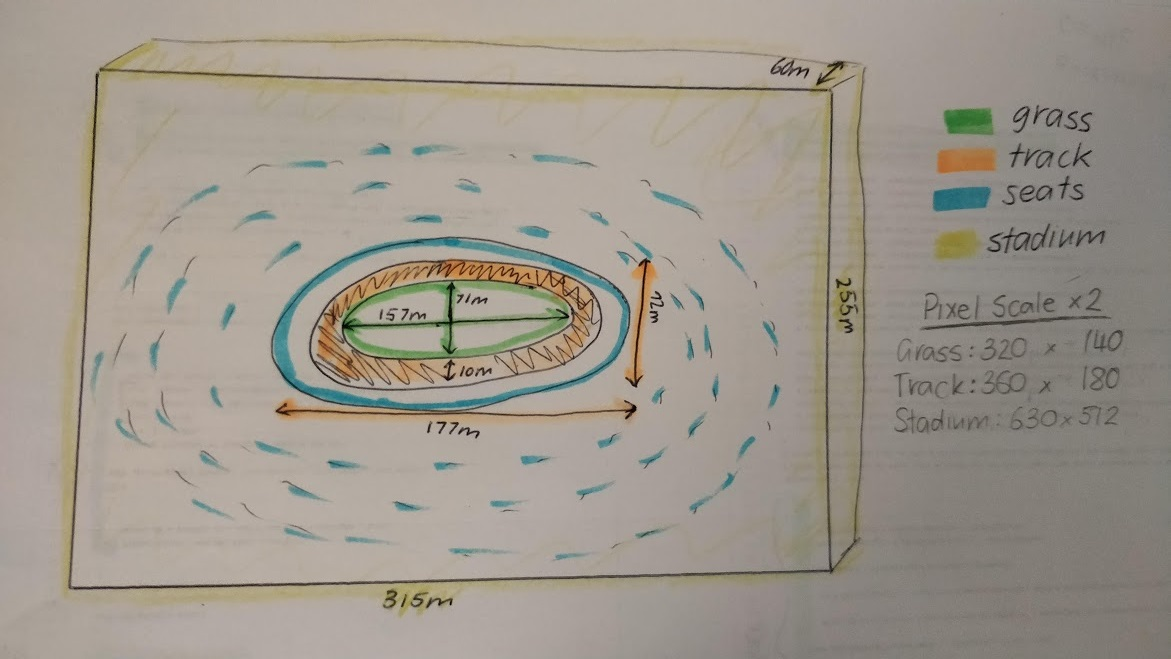
\includegraphics[width=0.8\textwidth, frame]
        {./images/olympics/track_dimensions.jpg}  
    \caption{Track - Olympic Stadium - Dimensions}   
\end{figure}

The track needed the 400m athletic track, grass in the entire of this track and then 6 levels of seating each 10m in height. With the basic layout and dimensional shape of the stadium set. The RGB colouring needed to be applied. Using the same setup, blue denoted the main channel (max speed), green the locations of object models and red the height.
    \begin{figure} [H]
        \centering
        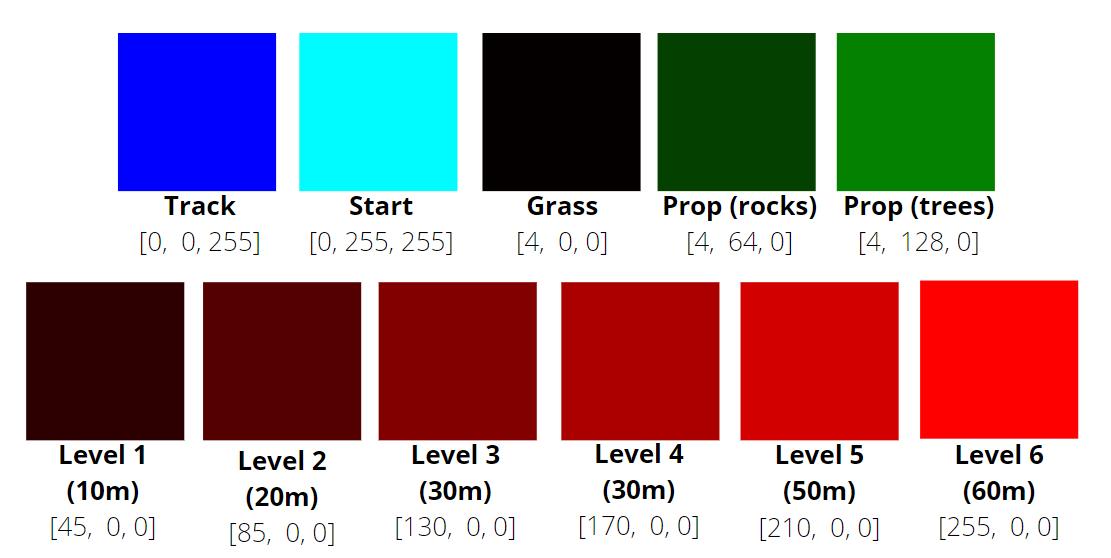
\includegraphics[width=0.8\textwidth, frame]
            {./images/olympics/track_colours.PNG}  
        \caption{Track - RGB Colours}   
    \end{figure}

Combining all of these together following track was produced to represents a stadium. The smoothness is definitely not ideal, and the sloping was difficult to duplicate. Though with access to only Paint and the low quality this was the best I could do. 
    \begin{figure} [H]
        \centering
        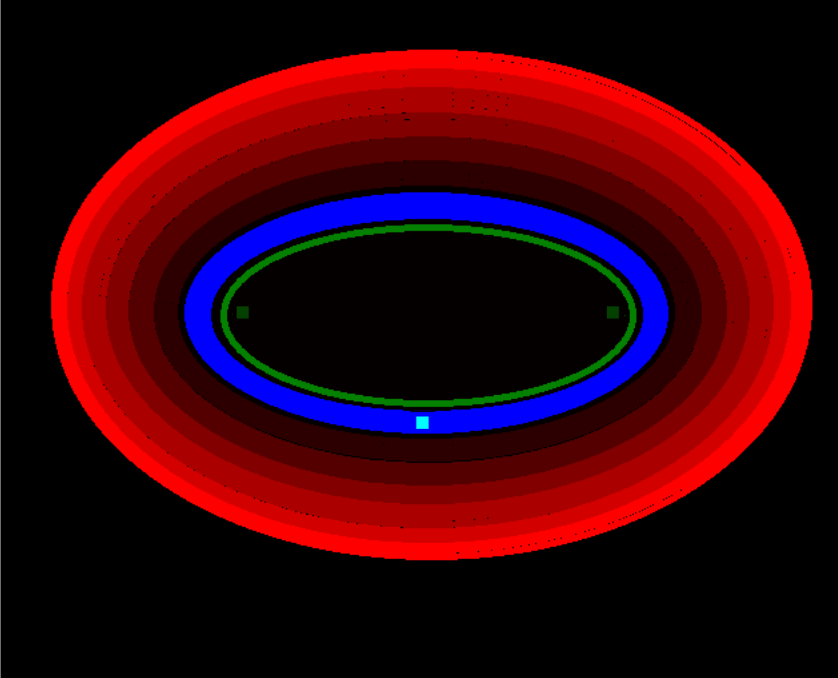
\includegraphics[width=0.8\textwidth, frame]
            {./images/olympics/track_final.PNG}  
        \caption{Track - Olympic Stadium - Final Track}   
    \end{figure}

    \begin{lstlisting}
#mega_racer.py    
g_terrain.load("data/track.png", g_renderingSystem);

# terrain.py
class Terrain:
    xyScale = 2
    heightScale = 60.0

    ....
    def load(...)
        ...    
        self.mapTexture = ObjModel.loadTexture("track.png", "data", False)
    \end{lstlisting}

\begin{figure} [H]
    \centering
    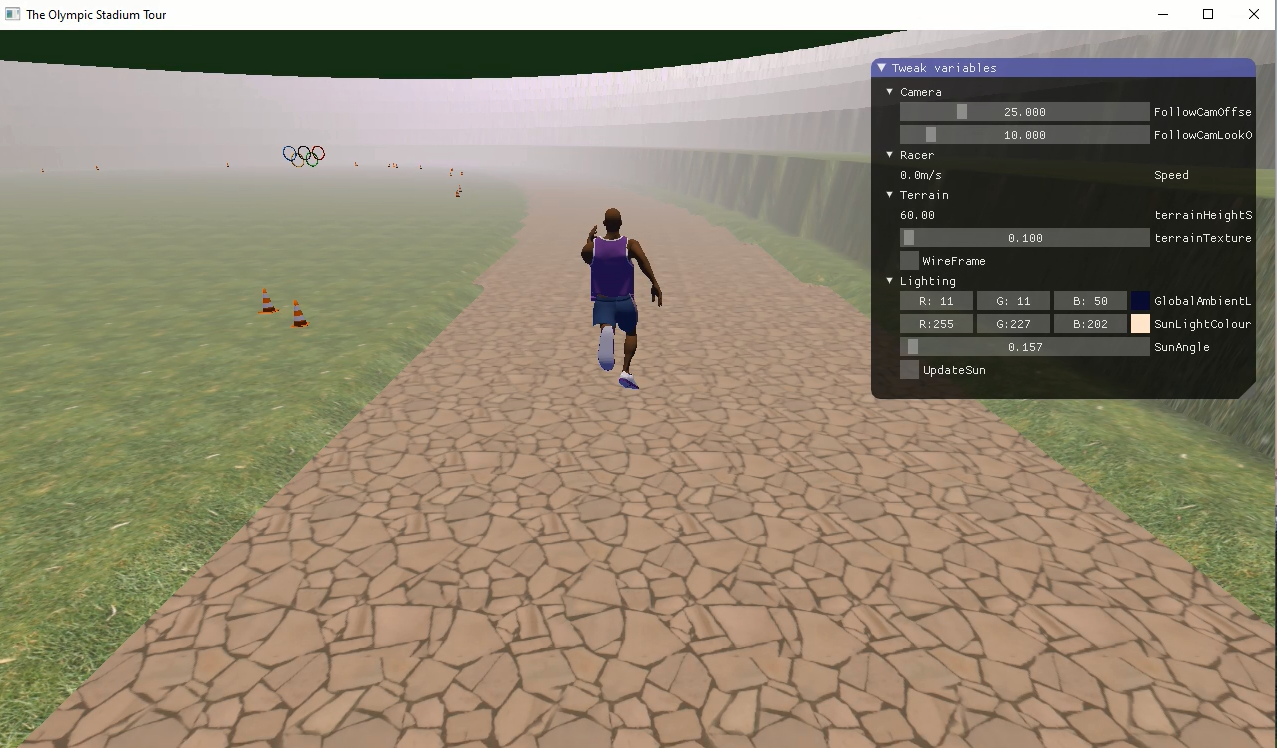
\includegraphics[width=0.8\textwidth, frame]
        {./images/olympics/map_world.PNG}  
    \caption{Track - RGB Colours}   
\end{figure}

% TERRAIN
\subsection{Terrain}
Finally, the textures of the terrain needed to be updated to reflect an Olympic Stadium. There were four textures to be implemented, as per the colouring on the map.
    \begin{enumerate}    
        \item Grass: This remained the same as mega\_racer, however a different 2D image was selected for the grassTexture. 
        \item Wall: This replaces the highTexture from mega\_racer. This texture is used to display a banner on the side wall, separating the athlete from the seating. This texture is only selected for the height of this wall, and the 2D image is a banner advertising the Tokyo 2020 Olympics.
        \item Seats: This replaces the steepTexture from mega\_racer. This texture is used for all areas above the height of the wall with a specific slope so that it only appears where there should be seating in the stands. This texture was the most disappointing and further adjustments to create more realistic seating would provide a more realistic appearance.
        \item Track: This replaces the road as the texture where the racer/athlete is at max speed. Instead of pavement the texture is a 2D image of red synthetic athletic track with a white line. Using the measurements from the map, an almost 8-lane track is visualised.
        \item Concrete: This is an additional texture that was added and replaces the grassTexture as the default texture. The 2D image is a simple concrete material that is used as the materialColour for all areas that do not meet the above logic.
    \end{enumerate}

    \begin{figure} [H]
        \centering
        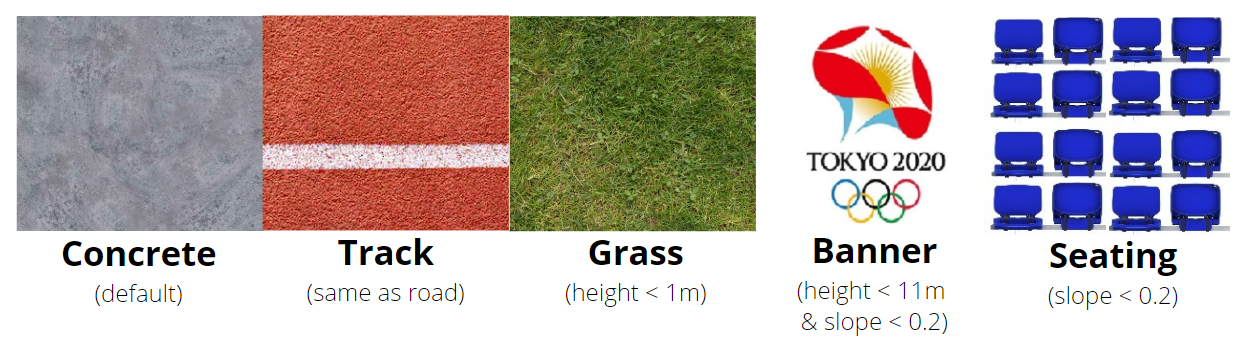
\includegraphics[width=0.8\textwidth, frame]
            {./images/olympics/terrain_textures.PNG}  
        \caption{Terrain - Textures}   
    \end{figure}

\begin{lstlisting} 
# terrain.py
class Terrain:
    ...
    textureXyScale = 0.25
    ...
    TU_Grass = 0
    TU_Wall = 1
    TU_Seats = 2
    TU_Track = 3   
    TU_Concrete = 5
    ...
    wallTexture = None
    seatsTexture = None
    trackTexture = None    
    concreteTexture = None
    ...

# terrain.py  
def render(...):
    ...
    lu.bindTexture(self.TU_Wall, self.wallTexture)
    lu.setUniform(self.shader, "wallTexture", self.TU_Wall)
    lu.bindTexture(self.TU_Seats, self.seatsTexture)
    lu.setUniform(self.shader, "seatsTexture", self.TU_Seats)
    lu.bindTexture(self.TU_Track, self.trackTexture)
    lu.bindTexture(self.TU_Map, self.mapTexture)
    lu.setUniform(self.shader, "trackTexture", self.TU_Track)
    lu.setUniform(self.shader, "mapTexture", self.TU_Map)
    lu.bindTexture(self.TU_Concrete, self.concreteTexture)
    lu.setUniform(self.shader, "concreteTexture", self.TU_Concrete)
    ...  
def load(...):
    ...
    self.wallTexture = ObjModel.loadTexture("banner.png", "data", True)
    self.seatsTexture = ObjModel.loadTexture("seats.png", "data", True)
    self.trackTexture = ObjModel.loadTexture("track.png", "data", True)
    self.mapTexture = ObjModel.loadTexture("track_edit5.png", "data", False)
    self.concreteTexture = ObjModel.loadTexture("concrete.jpg", "data", True)

# terrain.py 
fragmentShader = """
    ...
    uniform sampler2D wallTexture;
    uniform sampler2D seatsTexture;   
    uniform sampler2D trackTexture;
    uniform sampler2D mapTexture;
    uniform sampler2D concreteTexture;
    ...  
    void main() 
    void main() 
    {
        vec3 materialColour = vec3(v2f_height/terrainHeightScale);
        // Default colour 
        vec3 concreteColour = texture(concreteTexture, 
                        v2f_worldSpacePosition.xy * terrainTextureXyScale).xyz;
        materialColour = concreteColour;

        // 2.1                 
        float slope = dot(v2f_worldSpaceNormal, vec3(v2f_worldSpaceNormal.x, 0.0, 
                                                v2f_worldSpaceNormal.z)); //Steep 
        float blueChannel = texture(mapTexture, 
                                    (v2f_worldSpacePosition.xy - v2f_xyOffset) 
                                        * v2f_xyNormScale).z; //Road

        // Track Texture
        if (blueChannel >= 0.9) {
            vec3 trackColour = texture(trackTexture, v2f_worldSpacePosition.xy 
                                                    * terrainTextureXyScale).xyz;
            materialColour = trackColour;
        // Grass texture
        } else if (v2f_height < 1) {
            vec3 grassColour = texture(grassTexture, v2f_worldSpacePosition.xy 
                                                    * terrainTextureXyScale).xyz;
            materialColour = grassColour; 
        // Wall/Banner texture
        } else if ((v2f_height < 11) && (slope < 0.2)) {
            vec3 wallColour = texture(wallTexture, v2f_worldSpacePosition.xy 
                                                    * terrainTextureXyScale).xyz;
            materialColour = wallColour;                  
        // Seats
        } else if (slope < 0.2) {
            vec3 seatsColour = texture(seatsTexture, v2f_worldSpacePosition.xy 
                                                    * terrainTextureXyScale).xyz;
            materialColour = seatsColour; 
        }
        vec3 reflectedLight = computeShading(materialColour,  
                                            v2f_viewSpacePosition, 
                                            v2f_viewSpaceNormal, 
                                            viewSpaceLightPosition, 
                                            sunLightColour);
        fragmentColor = vec4(toSrgb(applyFog(reflectedLight, 
                                            -v2f_viewSpacePosition.z, 
                                            cameraPosition, 
                                            cameraToPointVector)), 1.0);
    }

    \end{lstlisting}

\begin{figure} [H]
    \centering
    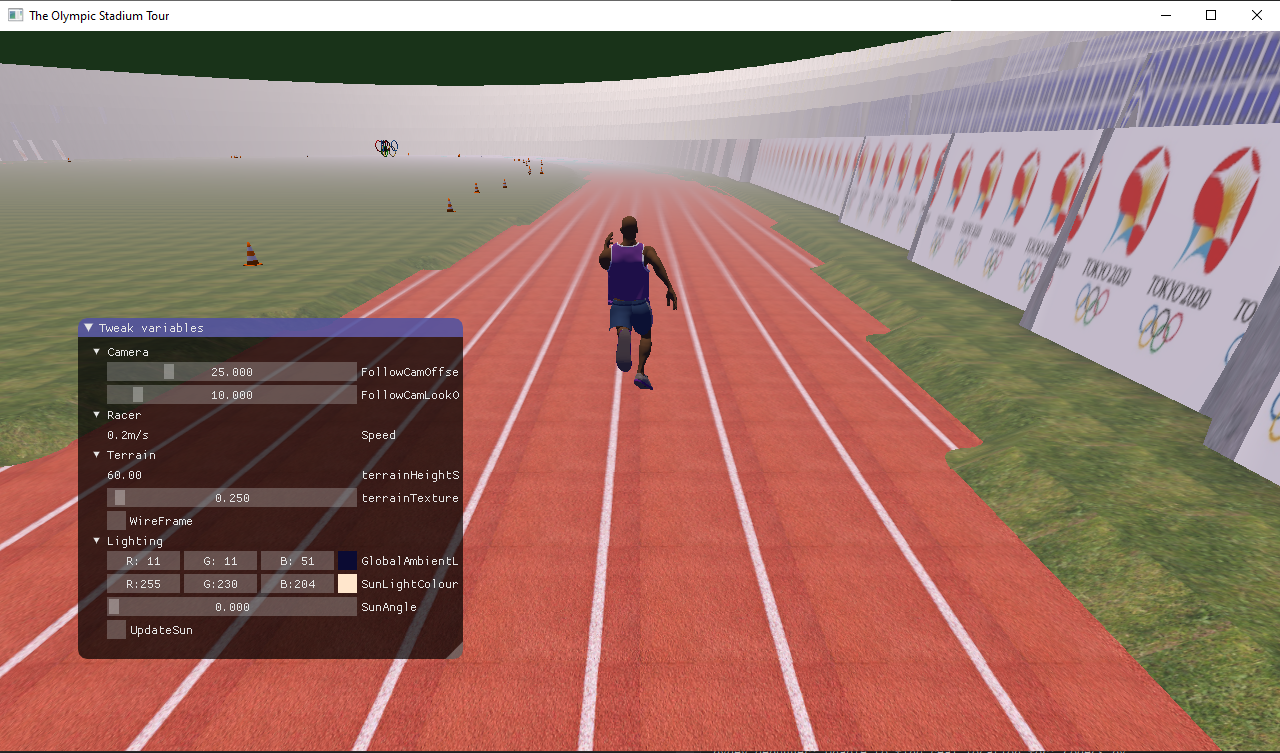
\includegraphics[width=0.8\textwidth, frame]
        {./images/olympics/terrain_world.PNG}  
    \caption{Terrain}   
\end{figure}


\section{Conclusion}
Throughout this project I have learnt, tested and successfully implemented a variety of Computer Graphics techniques to implement a basic version of the mega racer game and also a model of an Olympic Stadium. Concepts that were covered include coordinate systems, setting up a virtual camera, lighting, shading, texturing and modelling in Blender. All of the steps from the proposal were implemented except for structure of the stadium roof and its affect on shaping the lighting. There is always more than can be added and the next steps would be to create the roof using a cube mapping texture, more photorealistic skin texture on the athlete and a better visualisation of the stadium seating. Overall, an understanding of the gained knowledge of Computer Graphics concepts were demonstrated and communicated in this project.


\includepdf[pages=1, pagecommand=\section{References}, offset=0 0cm]{references.pdf}
\includepdf[pages=2-, offset=0 0cm]{references.pdf}
\end{document}